%====================================================
%	CHAPTER 6 - Control & Simulations
%====================================================
\chapter{Simulations and Results}
\label{ch:simulation}
%====================================================
\section{Simulator description}
\label{sec:simulation.block}
%====================================================
The proposed attitude and position control laws, together with the system's equations of motion including each actuator's transfer function, were all tested in simulation to determine a particular controller's efficacy. The rigid-body equations of motion from Sec:\ref{subsec:dynamics.rigidbody.lagrange}, with nonlinearities from Sec:\ref{sec:dynamics.aero} and multibody responses from Sec:\ref{sec:dynamics.nonlinearities}, were incorporated into a high fidelity simulation environment. Closely matching the dynamics of the physical quadrotor prototype proposed in Sec:\ref{sec:proto.design}; where measurement data produced by tests in Sec:\ref{subsec:dynamics.nonlinearities.torque-tests} provide a degree of confidence in the simulation's accuracy. The consolidated quaternion dynamics in Sec:\ref{sec:dynamics.model} formed the basis of the simulation, building a loop extended from the control structure in Fig:\ref{fig:control-block}. Each control law is optimized first without the effect of the servo's $180$\textdegree ~saturation limit. Limiting the servos was a conscious design decision, and so its effects are investigated in Sec:\ref{sec:simulation.saturation}. For now, the servos are treated as continuous rotational actuators without saturation limits.
\par
\begin{figure}[htbp]
\centering
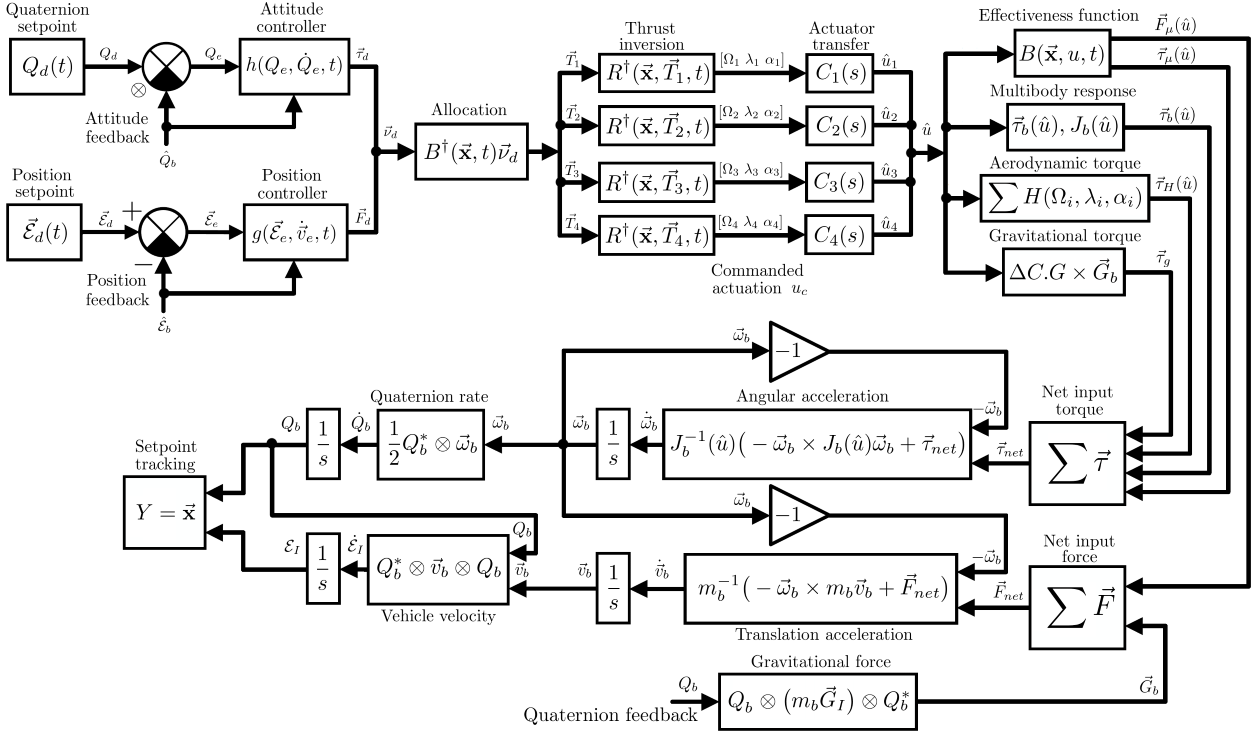
\includegraphics[width=\textwidth]{figs/simulation-block}
\vspace{-10pt}
\caption{Simulation loop}
\label{fig:simulation-block}
\end{figure}
\par
An abstracted simulation loop is illustrated in Fig:\ref{fig:simulation-block}, incorporating both attitude and position control loops together with the additive nonlinearities. Certain feedback elements were omitted to retain clarity in the diagram, both Coriolis and Gyroscopic nonlinear cross-products were included to highlight the inherent coupling between attitude and position. Not shown, but implied, is some form of state-estimation or discretization between the state-tracking output $y=\vec{\mathbf{x}}=[\vec{\mathcal{E}}_I~Q_b\hspace{2pt}]^T$ and the feedback state estimate $\hat{\mathbf{x}}$ used for setpoint tracking. Discretized effects of state-estimators are discussed later in Sec:\ref{sec:simulation.state}. Initial conditions for each state's integrator, both position $\vec{\mathcal{E}}_I(0)$ and attitude $Q_b(0)$ origins, for their velocities $\dot{\mathcal{E}}_b$ and $\dot{Q}_b$ (and accelerations $\dot{\vec{v}}_b$ and $\dot{\vec{\omega}}_b$ in the body frame $\mathcal{F}^b$) are not illustrated but implied. Obviously starting conditions are important for each trajectory's simulation but are specifically defined for each simulation in question. Actuator transfer functions from Sec:\ref{subsec:proto.design.transfer} are combined into a bundled $C_{i}(S)$ block, accounting for transfer functions and nonlinear saturation limits of each motor module. Each bundled input $u_{[1:4]}$ is similarly the projected actuator matrix:
\begin{equation}
u_i = \begin{bmatrix}
\Omega_i & \lambda_i & \alpha_i
\end{bmatrix}~~~~\text{for}~i\in[1:4]
\end{equation}
The resultant thrust vector $\vec{T}_i$ produced by each motor module has a net transfer function as a result of the propeller speed and servo rotation dynamics. Lastly, setpoints for both attitude and position states are either stepped or produced from an orbital trajectory. The former is used for controller optimization whilst the latter is used setpoint tracking performance evaluation. To discuss the question of non-zero setpoint tracking an orbital trajectory with an increasing orbital (\emph{chirp}) frequency generates attitude and position setpoints, illustrated in Fig:\ref{fig:trajectory}.
\begin{figure}[htbp]
\vspace{-10pt}
\centering
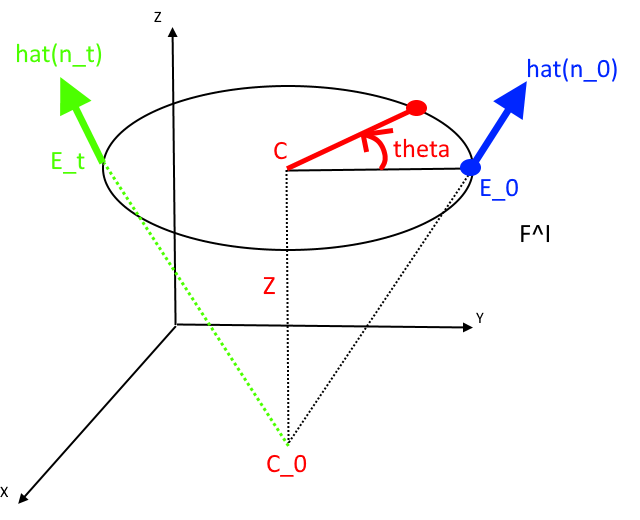
\includegraphics[width=0.9\textwidth]{figs/trajectory}
\vspace{-12pt}
\caption{Orbital trajectory}
\label{fig:trajectory}
\vspace{-20pt}
\end{figure}
\par
The trajectory generates only first order attitude and position setpoints, furthermore the trajectory setpoint is a body's attitude and inertial position, no actuator values for the aircraft's configuration are commanded by a trajectory. For a central point in the inertial frame $\vec{C}_0\in\mathcal{F}^I$, the trajectory orbits with a \emph{chirpyness} (frequency rate) of $\dot{\omega}~[\text{Hz.s}^{-1}]$ around that center. The orbit is at a height of $\hat{z}_c~[\text{m}]$ and at a radius $R_c~[\text{m}]$ from the center $\vec{C}$. The position setpoint then follows:
\begin{subequations}
\begin{equation}\label{eq:position-trajectory}
\vec{\mathcal{E}}_{d}(t)=\begin{bmatrix}
C_{0x}+R_c\cos\big(\dot{\omega}(t^2)\big)\\
C_{0y}+R_c\sin\big(\dot{\omega}(t^2)\big)\\
\hat{z}_c
\end{bmatrix}~~~~\in\mathcal{F}^I
\end{equation}
{\emph{\color{Gray}The frequency rate $\dot{\omega}$ used in Eq:\ref{eq:position-trajectory} describes the rate at which a chirp generated trajectory increases. It is not the same as an body's angular velocity $\vec{\omega}_b$. Convention has it that a signals frequency is annotated by $\omega$.}}
\par
The time varying trajectory's attitude setpoint is aligned with a normal vector $\hat{n}_d(t)$, banking the vehicle away from the center point $\vec{C}_0$:
\begin{equation}
\hat{n}_d(t)\triangleq\frac{\vec{\mathcal{E}}_d(t)-\vec{C}_0}{\sqrt{\hat{z}_c^2+R_c^2}}
\end{equation}
Using that normal $\hat{n}_d$ to construct a quaternion setpoint $Q_d(t)$ which varies together with the orbital trajectory:
\begin{equation}
Q_d(t)=\begin{bmatrix}
\sin \frac{\theta(t)}{2} & \cos \frac{\theta(t)}{2}\hat{n}_d(t)
\end{bmatrix}^T
\end{equation}
\end{subequations}
Whilst the trajectory equation itself may have a non-zero time derivative, both attitude and position controllers still apply the respective rate setpoints to the state variables $\dot{\vec{\mathcal{E}}}_d(t)=\vec{0}$ and $\dot{Q}_d(t)=\vec{0}$ throughout the entire trajectory, as per Eq:\ref{eq:4.85a} and Eq:\ref{eq:4.27c}. The plot in Fig:\ref{fig:Trajectory_Plot} shows a chirp quaternion and attitude trajectory, $Q_d(t)$ and $\vec{\mathcal{E}}_d(t)$ respectively, over a time period of $240~[\text{s}]$. The trajectory starts at $\vec{\mathcal{E}}_d(t_0)=[6~6~5]^T~[\text{m}]$, which produces a non-zero starting attitude $Q_d(t_0)=[0.38~0.42~0.24~0.7]^T$.\ref{fig:Position_Trajectory}.
\begin{figure}[htbp]
\vspace{-6pt}
\centering
\begin{subfigure}{\textwidth}
\centering
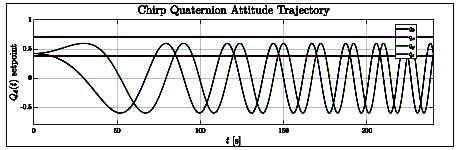
\includegraphics[width=0.8\textwidth]{graphs/Attitude_Trajectory}
\vspace{-6pt}
\caption{Quaternion setpoints}
\label{fig:Attitude_Trajectory}
\end{subfigure}
\begin{subfigure}{\textwidth}
\centering
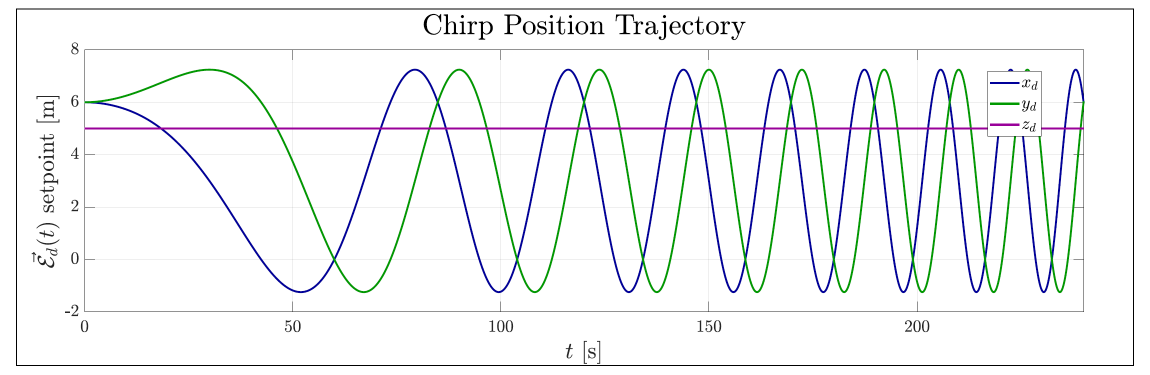
\includegraphics[width=0.8\textwidth]{graphs/Position_Trajectory}
\vspace{-6pt}
\caption{Position setpoints}
\label{fig:Position_Trajectory}
\end{subfigure}
\vspace{-8pt}
\caption{Chirp trajectory plots}
\label{fig:Trajectory_Plot}
\vspace{-12pt}
\end{figure}
%====================================================
\section{Controller Tuning}
\label{sec:simulation.tuning}
%====================================================
Each proposed control law's proven stability (in Sec:\ref{sec:control.attitude} and Sec:\ref{sec:control.position} for attitude and postition controllers respectively) demonstrates only a control law's setpoint tracking (error stability) for a time $t\rightarrow\infty$. That is the caveat with Lyapunov stability theorem, a trajectory is shown to be stabilizing, however no further insight into the controller coefficient design is provided. Often at the coefficient selection stage a \emph{Monte Carlo} approach is applied to select and optimize the controller coefficients.
%====================================================
\subsection{Particle Swarm Based Optimization}
\label{subsec:simulation.tuning.pso}
%====================================================
Particle swarm based optimization (\emph{PSO}) has been shown in both \cite{adaptivepso} and \cite{autopilotPSO}, amongst others, to be an effective controller coefficient design tool. The algorithm treats a potential set of controller coefficients as a single \emph{particle} which exists within some defined search space. The collection or \emph{swarm} of possible particles explores the search space directed by both the swarm's previous performance as well as the relative performance of the swarm between each particle. In \cite{particletrajectories} the statistical nature of the swarm's trajectory is discussed, however such investigations are beyond the scope of this work.
\par
In general, the PSO algorithm applies a \emph{gradient free} based search of solutions for a given optimization problem. The lack of a specified cost function gradient is an important distinction which differentiates PSO from other algorithms (note the swarm does update as per a pseudo-velocity function). Often a predefined cost function gradient is required to direct the optimization search at each interval, MatLab's fmincon\cite{fmincon} or Interior-Point optimizer\cite{ipopt} algorithms for example. Interval gradient calculations can be computationally exhaustive and reduce the rate of execution for the entire process. An optimizer's performance is directly proportional to the number of complete iterations it executes, if an iteration has a high degree of complexity (simulation \emph{stiffness}) its solution time is then adversely affected. The PSO algorithm is defined as follows: if there exists a set $\vec{x}$ of $k$ variables, $\vec{x}\in\mathbb{R}^{k\times 1}$ to be optimized. The swarm of particles, starting at particle $\vec{x}_0$, has an $n^{\text{th}}$ interval position $\vec{x}_n$ which progresses through the search space as per a velocity $\vec{v}_n$:
\begin{subequations}
\begin{equation}
\vec{x}_{n+1}=\vec{v}_{n}+x_{n}
\end{equation}
\vspace{-18pt}
\begin{equation}\label{eq:swarm-velocity}
\vec{v}_{n+1}\triangleq w\ast \vec{v}_n+c_1\ast r_1\big(\vec{P}_{best}-\vec{x}_n\big)+c_2\ast r_2\big(\vec{G}_{best}-\vec{x}_n\big)
\end{equation}
\end{subequations}
where each $\ast$ operator in Eq:\ref{eq:swarm-velocity} applies an element-by-element matrix coefficient multiplication. Both $\vec{P}_{best}$ and $\vec{G}_{best}$ are previous swarm positions where local and global optima were respectively achieved. Performance of the swarm's current interval is evaluated as per some cost function, responding to a system's dynamics. Finally $r_1$ and $r_2$ are random seeded $\mathbb{R}^{1\times k}$ exploratory matrices which progress the search direction, biased by the two weighting coefficients $c_1$ and $c_2$. The search is prejudiced toward local optima by $c_1$ whilst $c_2$ directs the swarm toward global optima. Fig:\ref{fig:swarm-trajectory} illustrates how positions of both local and global optima influence subsequent velocities.
\begin{figure}[hbtp]
\centering
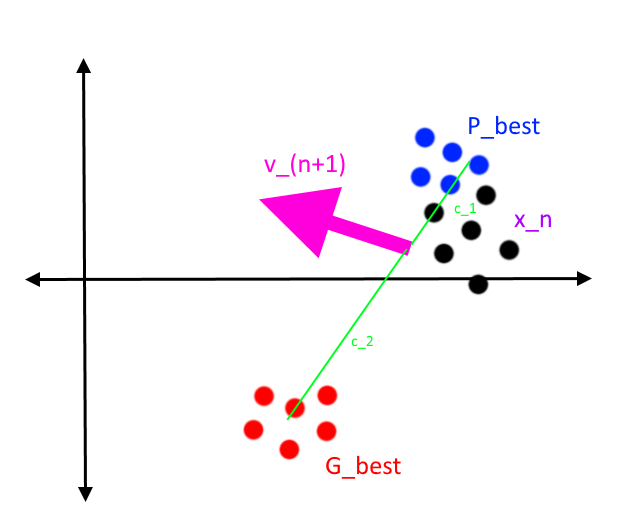
\includegraphics[width=0.8\textwidth]{figs/swarm-trajectory}
\vspace{-10pt}
\caption{Swarm trajectory's velocity direction}
\label{fig:swarm-trajectory}
\vspace{-8pt}
\end{figure}
\par
The swarm's interval performance is evaluated by the response of some modelled system to the swarm's position, typically an error deviation away from some desired state. Here, the simulation described in Fig:\ref{fig:simulation-block}, is parsed a swarm of controller coefficients as an argument and the plant's setpoint response is simulated over a series of step tests. Particulars with regards to attitude controller optimization is discussed in Sec:\ref{sec:simulation.attitude}, thereafter position controller optimization is detailed in Sec:\ref{sec:simulation.position}. The objective is for zero-error setpoint tracking so each particle's coefficient performance metric calculates an integral-time-absolute-error (\emph{ITAE}) cost function, \cite{ITAE}.
\begin{equation}
\vec{\zeta}\triangleq\int_{t_0}^{t_\infty}t||\vec{e}(t)||_2.dt
\end{equation}
With an error $\vec{e}(t)$ deviating from the plant's given setpoint. The ITAE integral $\vec{\zeta}$ is calculated over the entire simulation time, or an effective $t_\infty$. The time multiplier ensures setpoint error \emph{and} settling time optimality, punishing overshoot and under-damped or oscillatory like behavior. Generally a PSO algorithm progresses following the flow diagram in Fig:\ref{fig:particle-diagram}. Seeing that each controller was empirically proven to be stable irrespective of it's trajectory, the controller will settle irrespective of the proposed interval coefficient values. A consequence of this is that starting conditions $\vec{x}_0$ were chosen to be a rounded set of unity.
\\
\emph{\color{Gray} Note that $\vec{\mathbf{x}}$ is a state variable in the particle swarm flow diagram Fig:\ref{fig:particle-diagram}, $\vec{j}_n$ was chosen to represent the swarm of particles acted by the optimization algorithm in order to differentiate the two.}
\\
\begin{figure}[htbp]
\centering
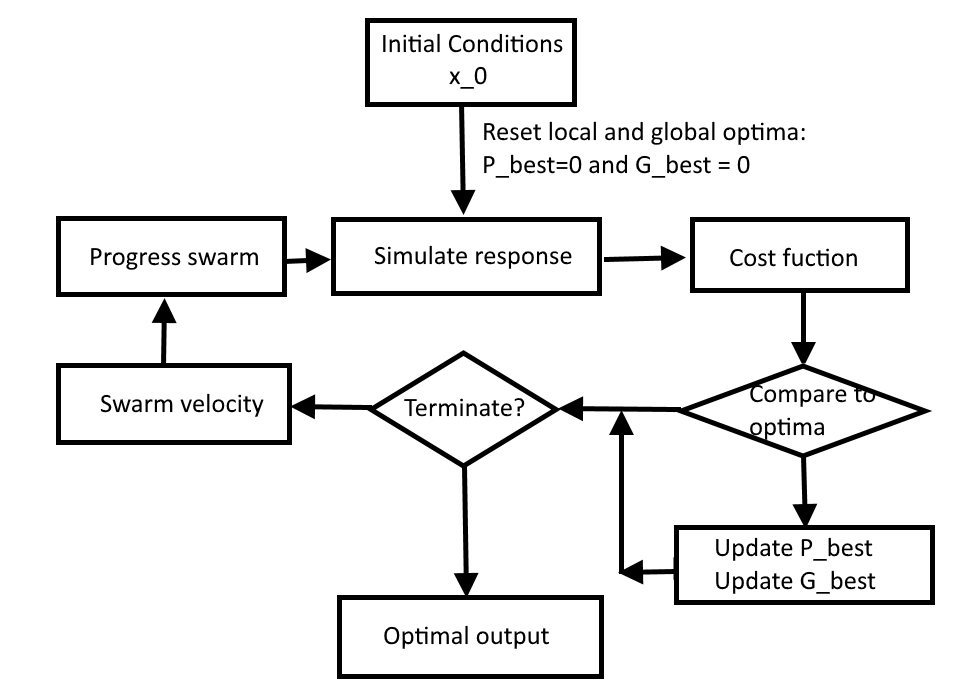
\includegraphics[width=0.8\textwidth]{figs/particle-diagram}\vspace{-12pt}
\caption{Particle swarm flow diagram}
\label{fig:particle-diagram}
\vspace{-18pt}
\end{figure}
\par
Termination conditions for the iterative optimization loop either limit the number of iteration cycles performed or break from the process once a result is regarded as sufficiently close to optimal. Each optimization loop was terminated only after a limited $tx=1000$ iterations, testing and evaluating one thousand different swarm values for a series of stepped setpoints. With control coefficients it is difficult to quantify how close to optimal a particular proposed set of coefficients are. As the optimizer progressed through iterations it adapted its bias coefficients $c_1$ and $c_2$ from focusing on global optima to local optima using fractions of the iteration number, refining the way in which it searched for potential controller coefficients.
\begin{equation}
\vec{v}_{n+1}=\vec{v}_n+\frac{tx}{1000}\ast r_1(\vec{P}_{best}-\vec{x}_n)+\frac{1000-tx}{1000}\ast r_2(\vec{G}_{best}-\vec{x}_n)~~~~\text{for}~~tx\in[1:1000]
\end{equation}
Each particle's progression was constrained such that it never violated the Lyapunov stability conditions of its respective control laws, mostly ensuring that the coefficient matrices were kept positive definite and symmetrical.
%====================================================
\section{Attitude Controllers}
\label{sec:simulation.attitude}
%====================================================
Attitude controllers derived in Sec:\ref{sec:control.attitude} were optimized first because of their lack of coupling with the position loop. The position control loop was left in open loop with only a constant hovering force condition applied to control input $\vec{F}_d$ for each test. Pseudo inverse allocation, Sec:\ref{subsec:allocation.allocators.inverse}, was applied to the control loop when testing each attitude controller. To evaluate an individual particle's performance a number of step tests were performed. Each attitude setpoint was first defined in the Euler angle parametrization, being conceptually easier to visualize. Thereafter the attitude setpoints were converted to a desired quaternion attitude and applied to the simulation.
\begin{equation}
\vec{\eta}_d(t)\triangleq \begin{bmatrix}
\phi_d(t)&
\theta_d(t)&
\psi_d(t)
\end{bmatrix}^T\underset{Q}{\iff}Q_d(t)
\end{equation}
Each of the three Euler angles were stepped in the range $[-90\text{\textdegree}:+90\text{\textdegree}]$ at intervals of $30\text{\textdegree}$. This resulted in a test of three hundred and forty three possible attitude setpoints, making a test-space sphere as illustrated in Fig:\ref{fig:attitude-setpoint}. Each attitude step was simulated for $t=15~[\text{s}]$ to allow its settling point, with an initial attitude position always set to the origin $Q_b(t_0)=[1~\vec{0}\hspace{2pt}]$, with a \emph{positive} quaternion scalar. The quaternion error's scalar component was limited to $q_0\in[0:1]$, detailed in Eq:\ref{eq:constrained-quaternion-error} of Sec:\ref{subsec:control.attitude.problem}, to ensure positive definite compatibility of the proposed Lyapunov candidate functions in the control proofs. The effect of an unconstrained, negative quaternion error scalar is illustrated in Fig:\ref{fig:PD_Quaternion_Step}. 
\par
Performance for each attitude step test was evaluated by an ITAE integral for the quaternion error vector and angular velocity error. Note that each gain coefficient in a particle has its own local and global error, so the performance metric $\vec{\zeta}_{q}$ is a \emph{vector}, not a scalar quantity:
\begin{equation}\label{eq:attitude-performance}
\vec{\zeta}_{Q}=\int_{t=0}^{15}C_Q*t*q_0*||\vec{q}_e(t)||.dt+\int_{t=0}^{15}C_\omega*t*||\vec{\omega}_e(t)||.dt~~~~\in\mathbb{R}^{3}
\end{equation}
Weighting coefficients $C_Q$ and $Q_\omega$ balance priority of either quaternion or angular velocity tracking, however, tracking both were equally important and so those weights were kept at unit with respective scalar units. The cost integral in Eq:\ref{eq:attitude-performance} was averaged over all three hundred and forty three possible attitude steps to determine the overall performance of a proposed swarm of controller coefficients.
\begin{figure}[htbp]
\vspace{-6pt}
\centering
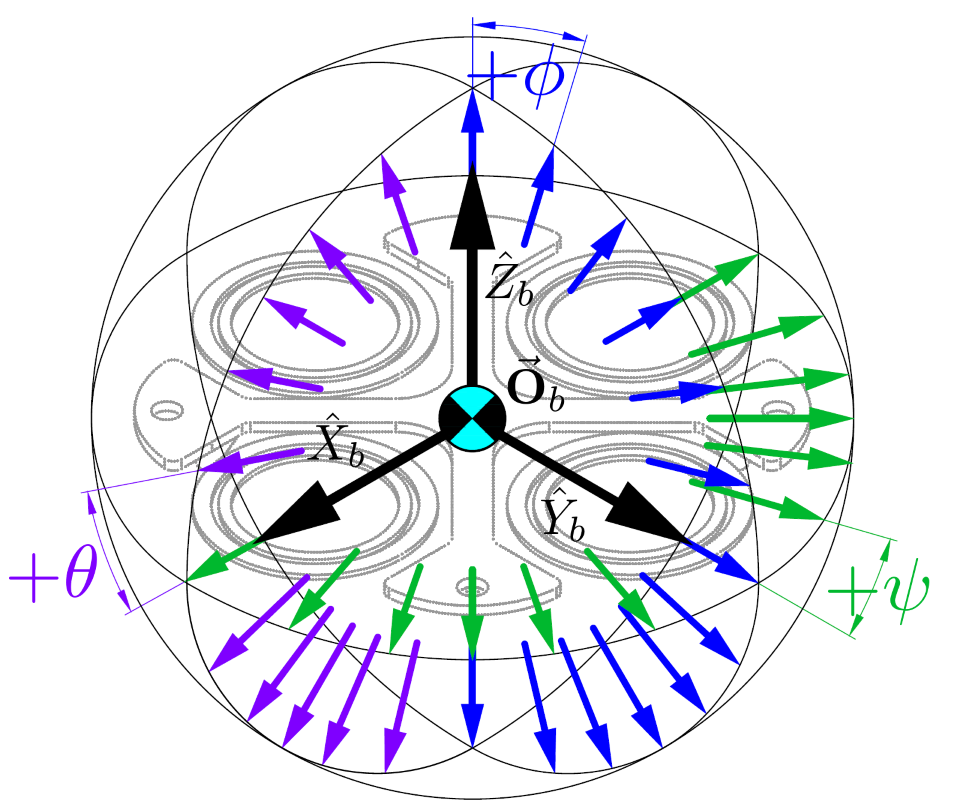
\includegraphics[width=0.72\textwidth]{figs/attitude-setpoint}
\vspace{-6pt}
\caption{Attitude setpoint working space}
\vspace{-14pt}
\label{fig:attitude-setpoint}
\end{figure}
\par
The integral in Eq:\ref{eq:attitude-performance} produces a $\mathbb{R}^{3}$ vector result. Each coefficient in a particular controller contributes towards a local error in one of the $\hat{X},\hat{Y},\hat{Z}$ components, or in certain cases a pair of axial components if the control coefficient is an off-diagonal element. A global error for the performance of each controller is simply the magnitude $||\vec{\zeta}_Q||$. The same global error is applicable to all controllers. 
\par
To compare the relative performance and effectiveness of each optimized control structure a single attitude step was investigated. That attitude change was chosen to be a sizable step in all three Euler angles to demonstrate the actuator dynamics' effect:
\begin{equation}\label{eq:attitude-step-position}
\vec{\eta}_d\triangleq\begin{bmatrix}
\phi_d\\
\theta_d\\
\psi_d\\
\end{bmatrix}
=
\begin{bmatrix*}[r]
-142\text{\textdegree}\\
167\text{\textdegree}\\
-45\text{\textdegree}
\end{bmatrix*}
\underset{Q}{\iff}
\begin{bmatrix}
-0.3254&
0.2226&
-0.2579&
0.8821
\end{bmatrix}^T
\end{equation}
Then each controller's settling time to $95$\% of its final value $t_{95}$ and its relative angular velocity (the setpoint $\vec{\omega}_d=\vec{0}$) for such a step is calculated. Settling time, overshoot and setpoint error are all factors to consider when discussing a controller's efficacy. Lastly, the commanded (virtual) and applied input torque to the actuator set are discussed too. A feasible controller should not induce torque saturation or unachievable input rate changes.
%====================================================
\subsection{PD}
\label{subsec:simulation.attitude.pd}
%====================================================
The first controller evaluated, the Proportional-Derivative structure, is investigated under three different circumstances. Before discussing each of different scenario, it is worth recalling that control structure from Sec:\ref{subsubsec:control.attitude.controllers.pd}. Control torque is designed by two coefficient matrices $K_p$ and $K_d$:
\begin{equation}\label{eq:simulation-attitde-pd}
\vec{\tau}_{_{PD}}=\underbrace{K_p\vec{q}_e+K_d\vec{\omega}_e}_{Independent}+\underbrace{\hat{\omega}_b\times J_b(\hat{u})\hat{\omega}_b+\vec{\tau}_b(\hat{u})-\vec{\tau}_g-\vec{\tau}_H}_{Compensation}~~~~\in\mathcal{F}^{b}
\end{equation}
The first two tests regard both coefficient matrices as purely diagonal, with no skew elements, testing the effect inclusion of plant dependent compensation has on the controller's performance. Finally a plant dependent compensating PD controller is tested \emph{with} symmetrical coefficient matrices. The diagonal coefficient matrices are defined as follows:
\begin{equation}\label{eq:simulation-attitde-pd-diagonal-coefficients}
K_p\triangleq \begin{bmatrix}
K_p(1) & 0 & 0\\
0 & K_p(2) & 0\\
0 & 0 & K_p(3)
\end{bmatrix}
~~\text{and}~~K_d\triangleq \begin{bmatrix}
K_d(1) & 0 & 0\\
0 & K_d(2) & 0\\
0 & 0 & K_d(3)
\end{bmatrix}
\end{equation}
The proportional coefficient $K_p$ acts on $\vec{q}_e$ whilst the derivative coefficient $K_d$ acts on $\vec{\omega}_e$, so local best positions are determined by elements of the error variable upon which each coefficient acts. A globally best position is tested simply with the magnitude $||\vec{z}_q||$ from Eq:\ref{eq:attitude-performance}. Then local and global best coefficient positions are updated if the minimum (best) result is improved on. 
\par
For the symmetrical coefficient case, each off-diagonal element acts on two components of the error states so then their local best positions depend on two elements of the error variables which they're related to. Then local and global coefficient positions are found when skew elements improve on \emph{two} combined error components. The  controller coefficients are structured:
\begin{equation}\label{eq:simulation-attitde-pd-symmetric-coefficients}
K_p\triangleq \begin{bmatrix}
K_p(1) & K_p(4) & K_p(5)\\
K_p(4) & K_p(2) & K_p(6)\\
K_p(5) & K_p(6) & K_p(3)
\end{bmatrix}
~~\text{and}~~K_d\triangleq \begin{bmatrix}
K_d(1) & K_d(4) & K_d(5)\\
K_d(4) & K_d(2) & K_d(6)\\
K_d(5) & K_d(6) & K_d(3)
\end{bmatrix}
\end{equation}
%====================================================
\subsubsection{Independent Performance}
\label{subsubsec:simulation.atttiude.pd.independent}
%====================================================
For the independent controller case, the same diagonal coefficients are used as those for the plant dependent case. The \emph{attitude} compensation terms in Eq:\ref{eq:simulation-attitde-pd} are neglected to produce a plant independent controller. 
\par
Optimizing the diagonal only PD controller produced the following coefficients:
\begin{equation}\label{eq:optimized-pd-independent}
K_p = \begin{bmatrix}
3.5679 & 0 & 0\\
0 & 5.2698 & 0\\
0 & 0 & 6.0695
\end{bmatrix}
~~\text{and}~~K_d = \begin{bmatrix}
9.0150 & 0 & 0\\
0 & 11.4848 & 0\\
0 & 0 & 20.1827
\end{bmatrix}
\end{equation}
Fig:\ref{fig:PD_Diagonal_Independent_Step} plots the quaternion response to an attitude step, described in Eq:\ref{eq:attitude-step-position}. The uncompensated plant never settles to its setpoint, constant steady state errors manifests due to the uncompensated gravitational and aerodynamic torques. The plant does, however, stabilize to steady state in $t = 3.35~\text{s}$. Fig:\ref{fig:PD_Diagonal_Independent_Torque} compares the controller designed and physically actuated input torques, $\vec{\tau}_d$ and $\vec{\tau}_c$ respectively. Actuator transfer functions produce a lagging response to those input changes. The body's angular velocity $\vec{\omega}_b\in\mathcal{F}^{b}$ is shown in Fig:\ref{fig:PD_Diagonal_Independent_Angular}, which changes as an attitude step is applied. Finally, Fig:\ref{fig:PD_Diagonal_Independent_Input} plots the motor modules' actuator inputs, still with sufficient input headroom from saturation despite such a large attitude step. The actuator servos for redirection of each module's produced thrust vector are, however, rate limited.
\\
\emph{\color{Gray}Note that module 2 and module 4 both anti-clockwise propeller directions, represented by negative speeds in Fig:\ref{fig:PD_Diagonal_Independent_Input}. }
\\
\begin{figure}[htbp]
\vspace{-22pt}
\centering
\begin{subfigure}{\textwidth}
\centering
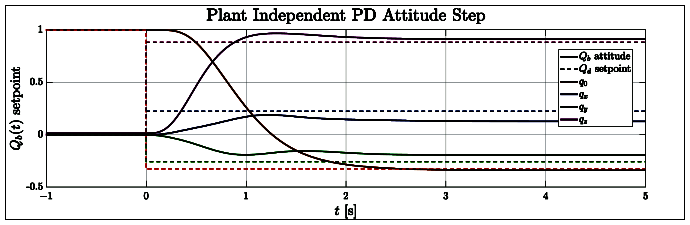
\includegraphics[width=0.7\textwidth]{graphs/PD_Diagonal_Independent_Step}
\vspace{-6pt}
\caption{Quaternion attitude step}
\label{fig:PD_Diagonal_Independent_Step}
\end{subfigure}
\begin{subfigure}{0.49\textwidth}
\centering
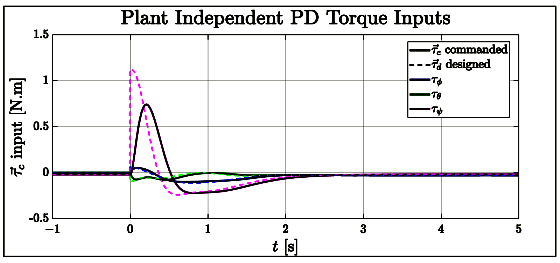
\includegraphics[width=\textwidth]{graphs/PD_Diagonal_Independent_Torque}
\vspace{-20pt}
\caption{Plant input torques}
\label{fig:PD_Diagonal_Independent_Torque}
\end{subfigure}
\begin{subfigure}{0.49\textwidth}
\centering
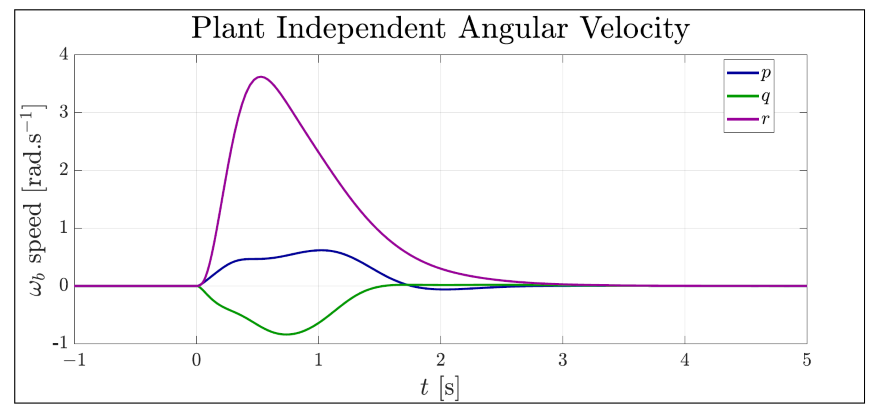
\includegraphics[width=\textwidth]{graphs/PD_Diagonal_Independent_Angular}
\vspace{-20pt}
\caption{Angular velocity}
\label{fig:PD_Diagonal_Independent_Angular}
\end{subfigure}
\begin{subfigure}{\textwidth}
\centering
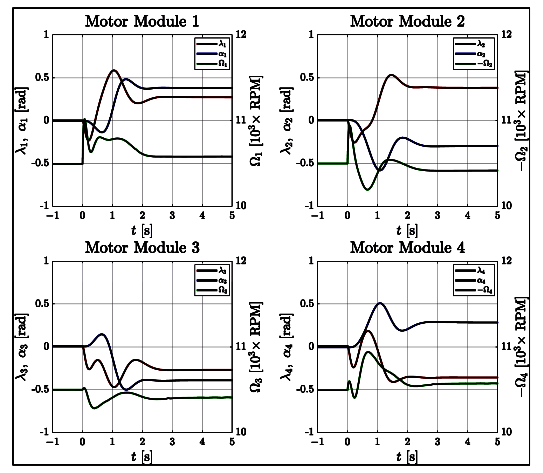
\includegraphics[width=0.6\textwidth]{graphs/PD_Diagonal_Independent_Input}
\vspace{-8pt}
\caption{Plant actuator inputs}
\label{fig:PD_Diagonal_Independent_Input}
\end{subfigure}
\vspace{-8pt}
\caption{Independent diagonal PD}
\vspace{-26pt}
\end{figure}
%====================================================
\subsubsection{Dependent Performance}
\label{subsubsec:simulation.atttiude.pd.dependent}
%====================================================
The inclusion of a plant independent PD controller is purely for the sake of comparison, indicating the need for plant dependency to account for steady state tracking errors (best illustrated with a trajectory test, later in Fig:\ref{fig:independent_diagonal_trjaectory}). The same controller coefficients from Eq:\ref{eq:optimized-pd-independent} were used to test the controller dependent case, where the controller accounts for plant dynamics in Eq:\ref{eq:simulation-attitde-pd} with feedback compensation.
\par
The standard quaternion attitude step applied in Fig:\ref{fig:PD_Diagonal_Dependent_Step} with plant dependent compensation. The attitude settles in $t_{95}=3.0764~\text{s}$ with a dynamic response much the same as that of the independent case, Fig:\ref{fig:PD_Diagonal_Independent_Step}. However the dependent controller removes steady state tracking errors. The only difference is that the plant dependent controller commands a non-zero steady state torque, illustrated by small increases in the servo actuator input rotations, shown in Fig:\ref{fig:PD_Diagonal_Dependent_Input}. It is interesting to note that the additional torque input is generated from redirection of the thrust vectors and not increasing or decreasing the propeller speeds.
\par
\begin{figure}[htbp]
\vspace{-10pt}
\centering
\begin{subfigure}{\textwidth}
\centering
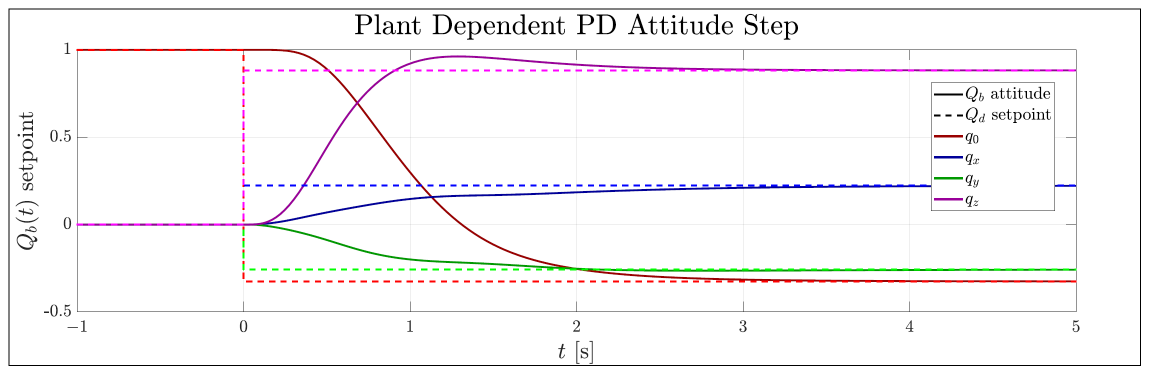
\includegraphics[width=0.7\textwidth]{graphs/PD_Diagonal_Dependent_Step}
\vspace{-6pt}
\caption{Quaternion attitude step}
\label{fig:PD_Diagonal_Dependent_Step}
\end{subfigure}
\begin{subfigure}{0.49\textwidth}
\centering
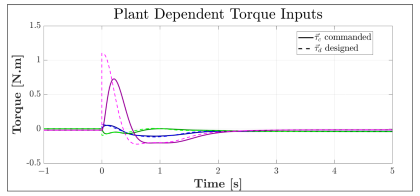
\includegraphics[width=\textwidth]{graphs/PD_Diagonal_Dependent_Torque}
\vspace{-20pt}
\caption{Plant input torques}
\label{fig:PD_Diagonal_Dependent_Torque}
\end{subfigure}
\begin{subfigure}{0.49\textwidth}
\centering
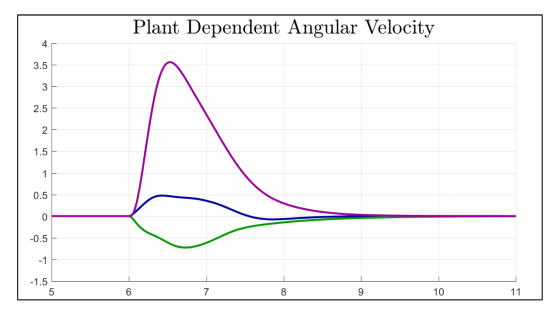
\includegraphics[width=\textwidth]{graphs/PD_Diagonal_Dependent_Angular}
\vspace{-20pt}
\caption{Angular velocity}
\label{fig:PD_Diagonal_Dependent_Angular}
\end{subfigure}
\begin{subfigure}{\textwidth}
\centering
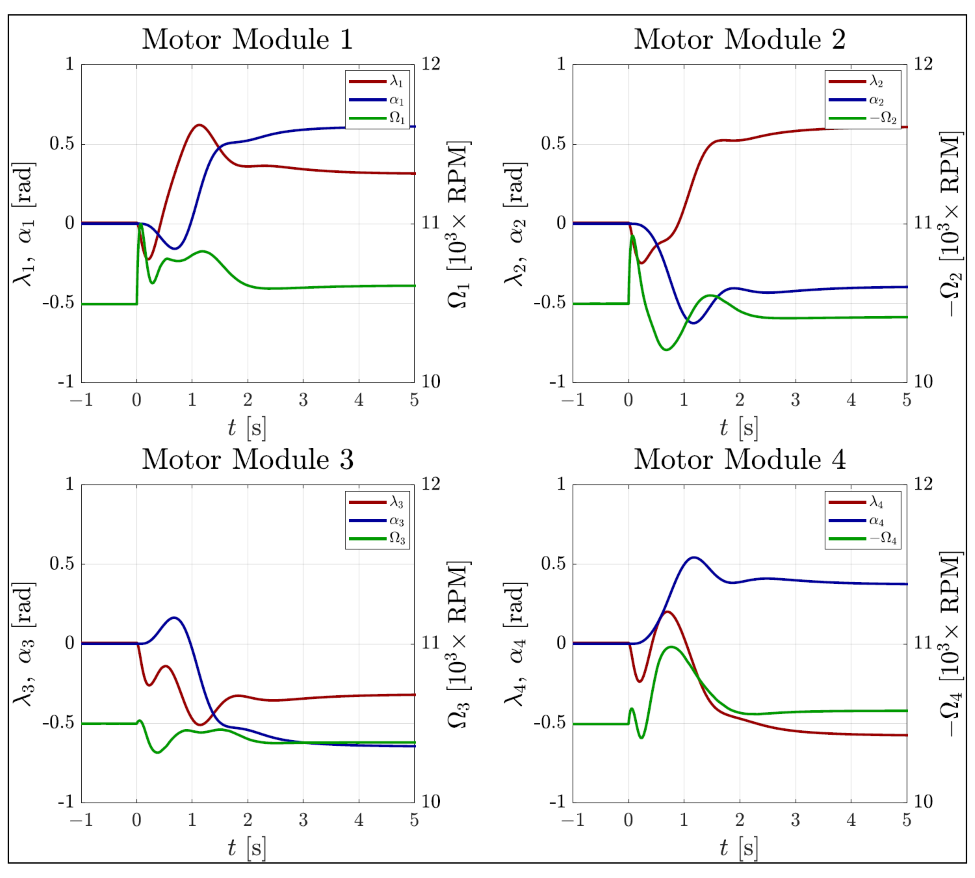
\includegraphics[width=0.6\textwidth]{graphs/PD_Diagonal_Dependent_Input}
\vspace{-8pt}
\caption{Plant actuator inputs}
\label{fig:PD_Diagonal_Dependent_Input}
\end{subfigure}
\vspace{-8pt}
\caption{Dependent diagonal PD}
\vspace{-26pt}
\end{figure}
%====================================================
\subsubsection{Symmetric Controller Performance}
\label{subsubsec:simulation.atttiude.pd.3x3}
%====================================================
The last PD structured attitude controller considers both coefficient matrices with non-zero off-diagonal skew elements. Eq:\ref{eq:simulation-attitde-pd-symmetric-coefficients} shows the structure of both symmetric matrices whose optimized coefficients were found to be:
\begin{equation}\label{eq:optimized-pd-symmetric}
K_p = \begin{bmatrix*}[l]
5.9157 & 0.4165 & 0.4714\\
0.4165 & 7.3141 & 0.4945\\
0.4714 & 0.4945 & 7.3135
\end{bmatrix*}
~~\text{and}~~K_d = \begin{bmatrix*}[l]
17.4318 & 0.45311 & 0.15258\\
0.45311 & 15.3569 & 0.57719\\
0.15258 & 0.57719 & 26.3436
\end{bmatrix*}
\end{equation}
The biggest change the symmetric controller imposes is greater controller gain, $||K_p||_2$ abd $||K_d||_2$ applied to quaternion and angular velocity errors. The increased gain in Eq:\ref{eq:optimized-pd-symmetric} results in larger overshoot and, as a result, slower settling time $t_{95}=3.2993~[\text{s}]$. Neither greater commanded torque, Fig:\ref{fig:PD_3x3_Dependent_Torque}, nor an increased angular velocity spike, Fig:\ref{fig:PD_3x3_Dependent_Angular} are unexpected consequences of a more aggressive control law. More coefficients to be tuned simply meant that optimization intervals to produce Eq:\ref{eq:optimized-pd-symmetric} were perhaps not as effective at reduction of step errors than the diagonal Eq:\ref{eq:optimized-pd-independent}.
\begin{figure}[htbp]
\vspace{-10pt}
\centering
\begin{subfigure}{\textwidth}
\centering
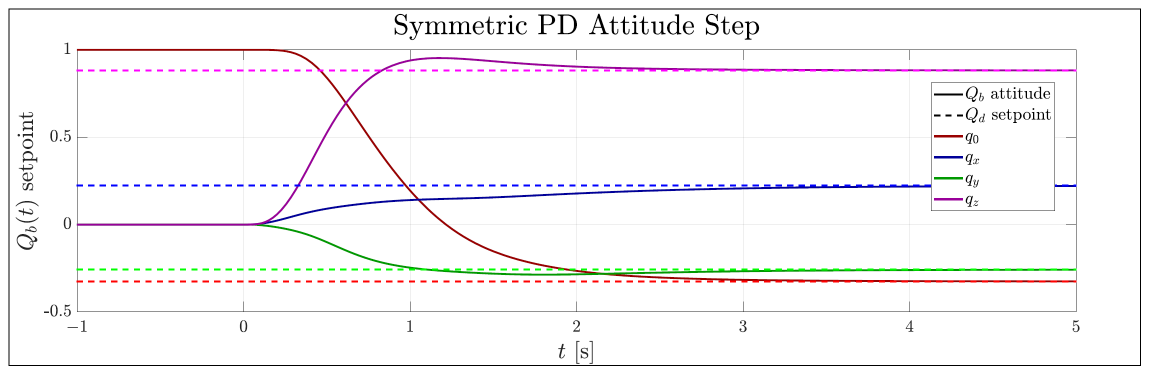
\includegraphics[width=0.7\textwidth]{graphs/PD_3x3_Dependent_Step}
\vspace{-6pt}
\caption{Quaternion attitude step}
\label{fig:PD_3x3_Dependent_Step}
\end{subfigure}
\begin{subfigure}{0.49\textwidth}
\centering
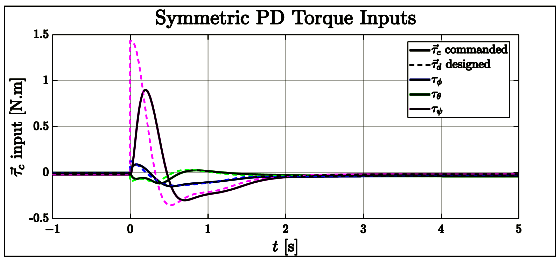
\includegraphics[width=\textwidth]{graphs/PD_3x3_Dependent_Torque}
\vspace{-20pt}
\caption{Plant input torques}
\label{fig:PD_3x3_Dependent_Torque}
\end{subfigure}
\begin{subfigure}{0.49\textwidth}
\centering
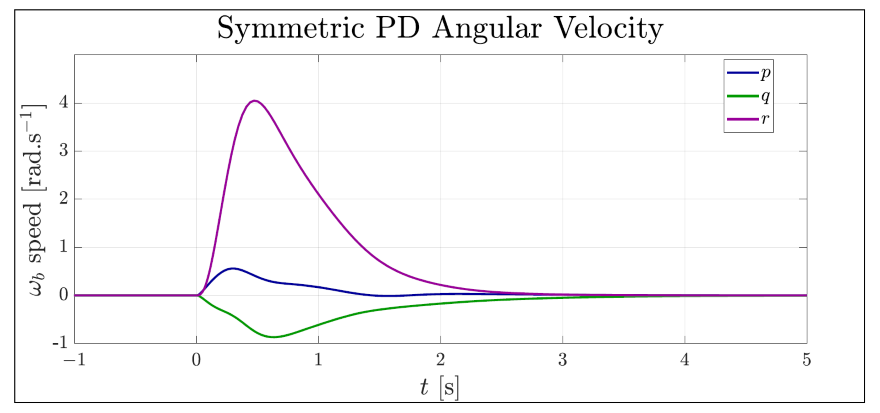
\includegraphics[width=\textwidth]{graphs/PD_3x3_Dependent_Angular}
\vspace{-20pt}
\caption{Angular velocity}
\label{fig:PD_3x3_Dependent_Angular}
\end{subfigure}
\begin{subfigure}{\textwidth}
\centering
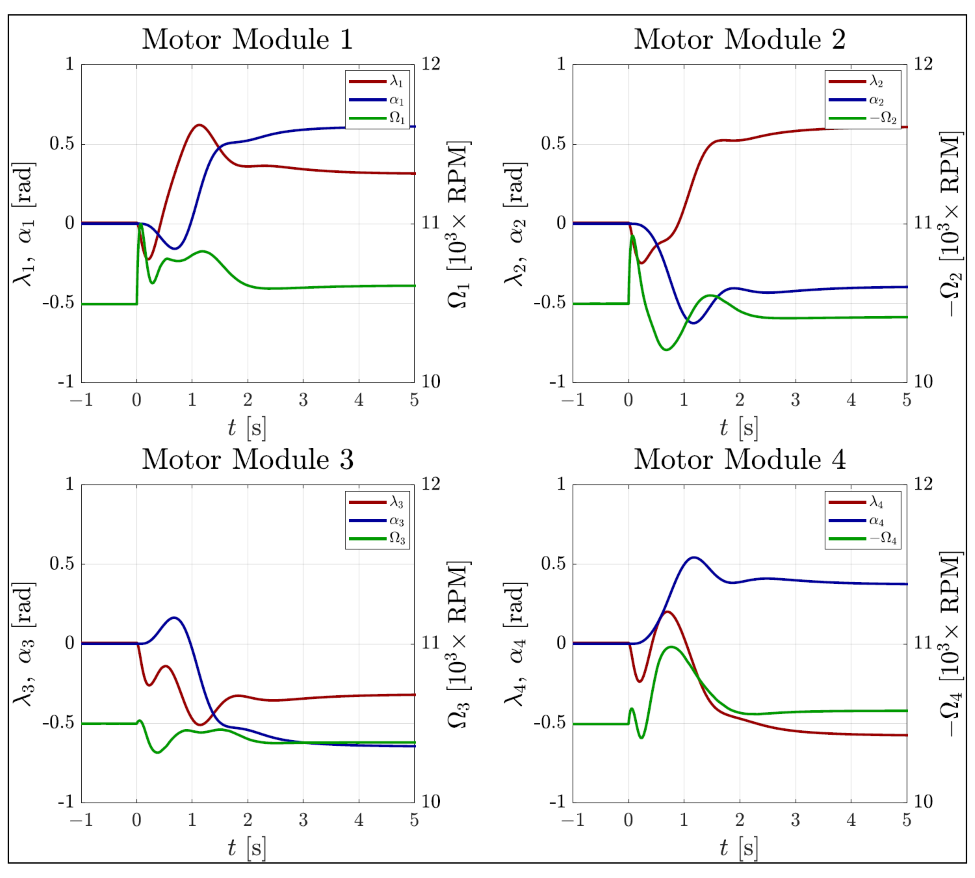
\includegraphics[width=0.6\textwidth]{graphs/PD_Diagonal_Dependent_Input}
\vspace{-8pt}
\caption{Plant actuator inputs}
\label{fig:PD_3x3_Dependent_Input}
\end{subfigure}
\vspace{-8pt}
\caption{Dependent symmetric PD}
\vspace{-26pt}
\end{figure}
\par
The $[3\times 3]$ symmetric controller's coefficients in Eq:\ref{eq:optimized-pd-symmetric} demonstrate that improving a controller's performance is not as simple as just increasing the controller's gain. To that end, consider the diagonal plant dependent PD controller previously in Sec:\ref{subsubsec:simulation.atttiude.pd.dependent}. If the gain is increased by a scale factor of 2, the settling time decreases to $t_{95}=6.8017~[\text{s}]$ from $t_{95}=3.0764~[\text{s}]$. The attitude step for a PD controller with an increased gain is shown in Fig:\ref{fig:PD_Diagonal_Gain_Step}, with actuator inputs shown in Fig:\ref{fig:PD_Diagonal_Gain_Input}. More gain does not necessarily mean a faster controller.
\begin{figure}[htbp]
\vspace{-10pt}
\centering
\begin{subfigure}{\textwidth}
\centering
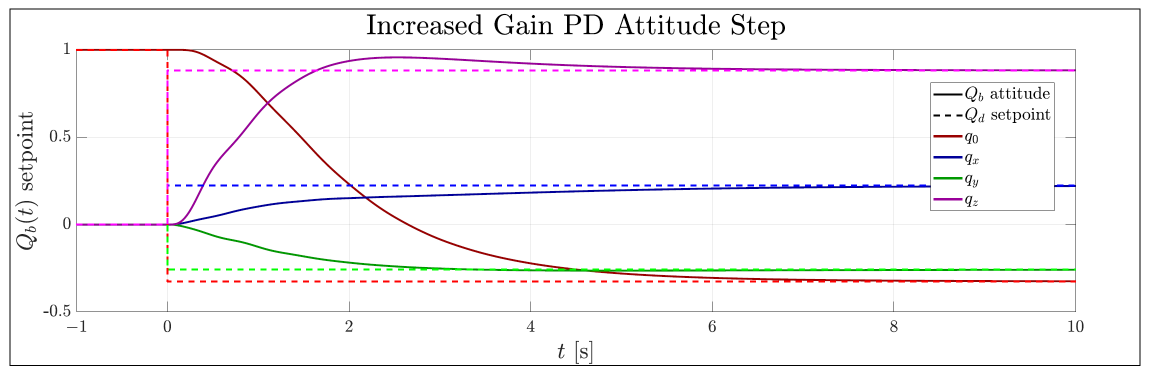
\includegraphics[width=0.7\textwidth]{graphs/PD_Diagonal_Gain_Step}
\vspace{-6pt}
\caption{Quaternion attitude step}
\label{fig:PD_Diagonal_Gain_Step}
\end{subfigure}
\begin{subfigure}{\textwidth}
\centering
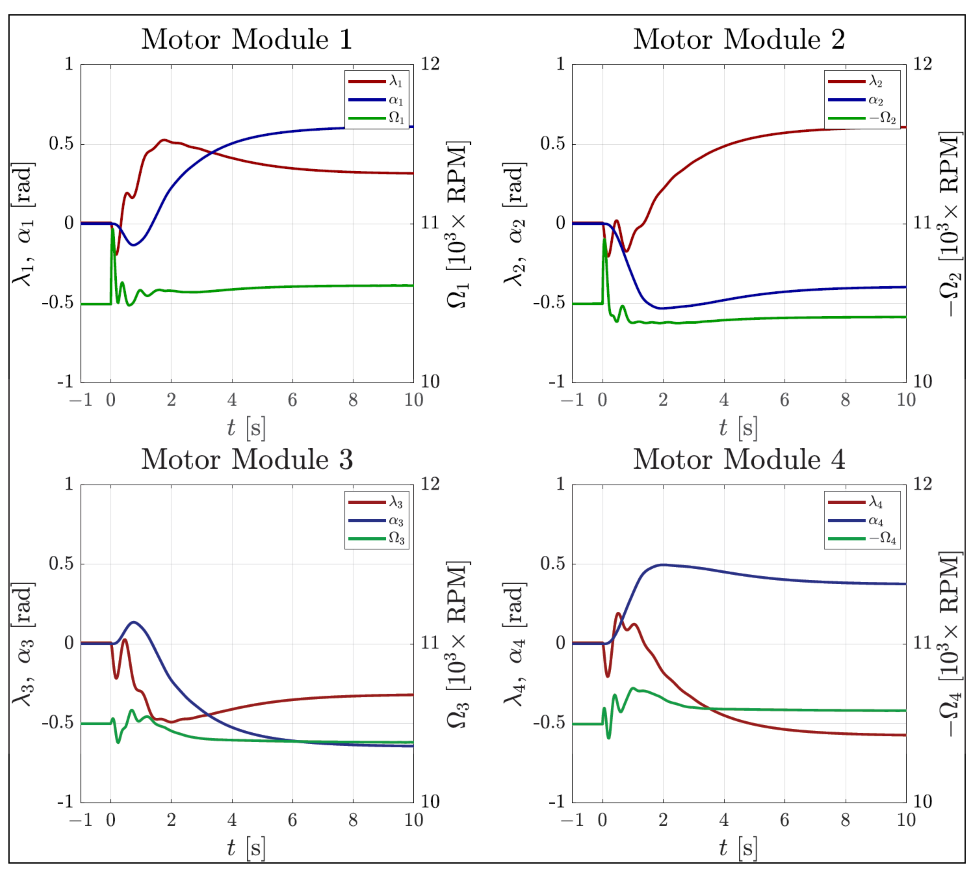
\includegraphics[width=0.6\textwidth]{graphs/PD_Diagonal_Gain_Input}
\vspace{-8pt}
\caption{Plant actuator inputs}
\label{fig:PD_Diagonal_Gain_Input}
\end{subfigure}
\vspace{-8pt}
\caption{Increased gain PD}
\vspace{-16pt}
\end{figure}
\par
It is worth discussing the constrained quaternion error's scalar limited to $q_0\in[0:1]$. That constraint was imposed during the control stability proof (Sec:\ref{subsec:control.attitude.problem}) where the constrained quaternion ensured that each proposed Lyapunov function candidate was always positive definite. Commanding the same quaternion step from Eq:\ref{eq:attitude-step-position}, however using the negative counterpart of the quaternion error's scalar  $q_0\in[-1:0]$, gives a step response shown in Fig:\ref{fig:PD_Quaternion_Step}. No difference is produced from using $Q_e=[\pm q_0~\vec{q}_e]^T$, despite the requirements of the stability proof. A positive definite LFC \emph{ensures} suitable stability but is by no means the \emph{only condition} at which stability is achieved.
\begin{figure}[hbtp]
\centering
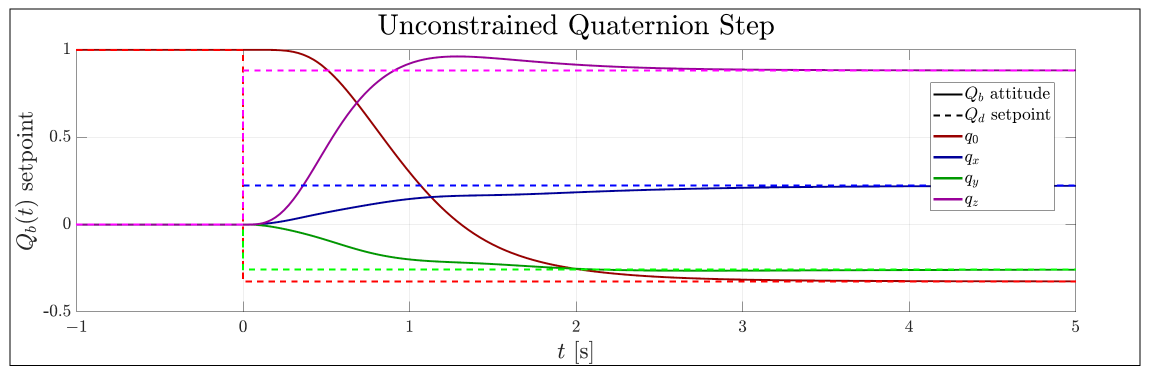
\includegraphics[width=0.7\textwidth]{graphs/PD_Unconstrained_Step}
\vspace{-6pt}
\caption{Unconstrained Error Quaternion attitude step}
\label{fig:PD_Quaternion_Step}
\vspace{-10pt}
\end{figure}
%====================================================
\subsection{Auxiliary Plant Controller}
\label{subsec:simulation.attitude.xpd}
%====================================================
The first of two the exponentially stabilizing controllers is the auxiliary Plant controller from Sec:\ref{subsubsec:control.attitude.controllers.auxpd}. Recalling that controller structure from Eq:\ref{eq:control-aux-pd}:
\begin{subequations}
\begin{equation}\label{eq:simulation-attitude-auxpd}
\vec{\tau}_{_{XPD}}=\underbrace{\Gamma_2{\widetilde{\Omega}}+\Gamma_3\vec{q}_e-J_b(\hat{u})\dot{\bar{\Omega}}}_{Independent}+\underbrace{\hat{\omega}_b\times J_b(\hat{u})\hat{\omega}_b+\vec{\tau}_b(\hat{u})-\vec{\tau}_g-\vec{\tau}_H}_{Compensation}~~~~\in\mathcal{F}^{b}
\end{equation}
where the auxiliary signals $\widetilde{\Omega}$ and $\bar{\Omega}$ are defined, from Eq:\ref{eq:aux-pd-1} and Eq:\ref{eq:aux-pd-2} respectively, as:
\begin{equation}
\bar{\Omega}\triangleq - \Gamma_1\vec{q}_e~~\text{and}~~\widetilde{\Omega}\triangleq -\vec{\omega}_b-\bar{\Omega}
\end{equation}
\end{subequations}
In Eq:\ref{eq:simulation-attitude-auxpd} both coefficients $\Gamma_2$ and $\Gamma_3$ are $[3\times 3]$ diagonal coefficient matrices, whilst $\Gamma_1$ is a symmetrical $[3\times 3]$ gain matrix. Those coefficients are then structured as follows:
\begin{multline}\label{eq:simulation-attitde-auxpd-coefficients}
\Gamma_1\triangleq \begin{bmatrix}
\Gamma_1(1) & \Gamma_1(4) & \Gamma_1(5)\\
\Gamma_1(4) & \Gamma_1(2) & \Gamma_1(6)\\
\Gamma_1(5) & \Gamma_1(6) & \Gamma_1(3)
\end{bmatrix}~,~~
\Gamma_2\triangleq \begin{bmatrix}
\Gamma_2(1) & 0 & 0\\
0 &\Gamma_2(2) & 0\\
0 & 0 & \Gamma_2(3)
\end{bmatrix}
\\
~~\text{and}~~\Gamma_3\triangleq \begin{bmatrix}
\Gamma_3(1) & 0 & 0\\
0 & \Gamma_3(2) & 0\\
0 & 0 & \Gamma_3(3)
\end{bmatrix}
\end{multline}
Global and local best positions of coefficient particles are found from the error state components on which the particular coefficients act. The first gain matrix $\Gamma_1$ acts on both $\vec{q}_e$ and $\vec{\omega}_e$, so its local best position $\vec{P}_{best}$ is when both errors are at their minimum. The remaining two gain matrices $\Gamma_2$ and $\Gamma_3$ act on $\vec{q}_e$ and $\vec{\omega}_e$ respectively, so their local best positions are when each of those errors are minimized. And finally the globally best performing particle position is when $||\vec{\zeta}||_2$ is minimized. The control coefficients produced after $tx=1000$ iterations are as follows:
\begin{multline}\label{eq:optimized-auxpd}
\Gamma_1=\begin{bmatrix*}[r]
3.5924 & -0.2457 & -0.0277\\
-0.2457 & 3.0666 & -0.0602\\
-0.0277 & -0.0602 & 3.3809
\end{bmatrix*}~,~~\Gamma_2=\begin{bmatrix*}[r]
4.6943 & 0 & 0\\
0 & 4.1642 & 0\\
0 & 0 & 6.4109
\end{bmatrix*}\\
~~\text{and}~~\Gamma_3=\begin{bmatrix*}[r]
1.1007 & 0 & 0\\
0 & 1.3369 & 0 \\
0 & 0 & 1.1331
\end{bmatrix*}
\end{multline}
Besides from the stronger exponential stability, another distinctive feature of auxiliary Controller (Eq:\ref{eq:simulation-attitde-auxpd-coefficients}) is the introduced simulation stiffness to the control structure. Calculations for the control input at each interval became more complex as a result of the introduced error terms. Each iteration of the optimizer took longer to simulate, typically in the order of 70-80\% longer, per step test.
\par
The quaternion attitude step response is shown in Fig:\ref{fig:XPD_Step}, settling in $t_{95}=2.3688~\text{s}$ which is notably faster than previous tested controllers. The improved response time does, however, come at the cost of greater input torques, shown in Fig:\ref{fig:XPD_Torque}. Moreover commanded angular velocity change in $\vec{\omega}_b$ (Fig:\ref{fig:XPD_Angular}) is markedly larger than that of previous controllers.
\begin{figure}[hbtp]
\vspace{-8pt}
\centering
\begin{subfigure}{\textwidth}
\centering
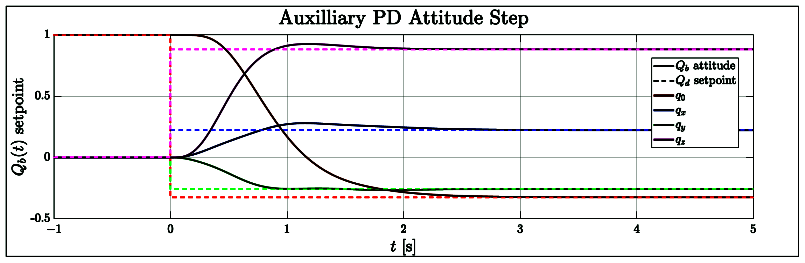
\includegraphics[width=0.7\textwidth]{graphs/XPD_Step}
\vspace{-6pt}
\caption{Quaternion attitude step}
\label{fig:XPD_Step}
\end{subfigure}
\vspace{-14pt}
\end{figure}
\newpage
\begin{figure}[htbp]\ContinuedFloat
\begin{subfigure}{0.49\textwidth}
\centering
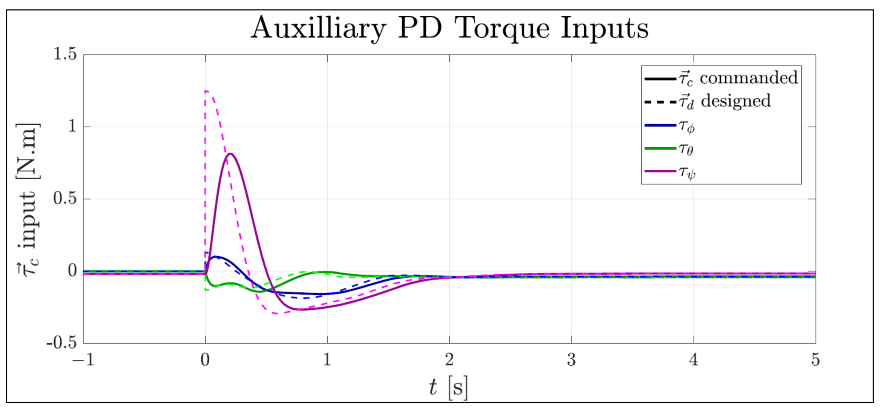
\includegraphics[width=\textwidth]{graphs/XPD_Torque}
\vspace{-20pt}
\caption{Plant input torques}
\label{fig:XPD_Torque}
\end{subfigure}
\begin{subfigure}{0.49\textwidth}
\centering
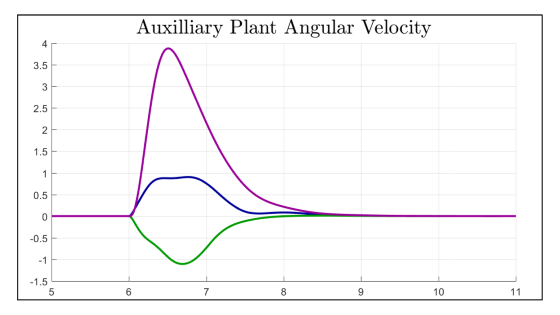
\includegraphics[width=\textwidth]{graphs/XPD_Angular}
\vspace{-20pt}
\caption{Angular velocity}
\label{fig:XPD_Angular}
\end{subfigure}
\begin{subfigure}{\textwidth}
\centering
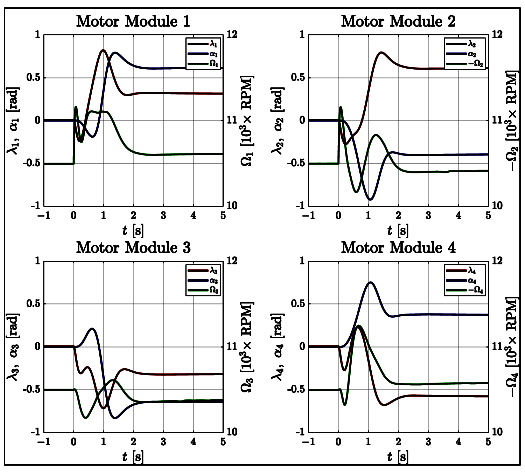
\includegraphics[width=0.6\textwidth]{graphs/XPD_Input}
\vspace{-6pt}
\caption{Plant actuator inputs}
\label{fig:XPD_Input}
\end{subfigure}
\vspace{-8pt}
\caption{Auxiliary Plant PD}
\end{figure}
Despite the improved (23\% faster) settling time the auxiliary PD controller achieves, neither the applied torque inputs (Fig:\ref{fig:XPD_Torque}) nor the actuator commands (Fig:\ref{fig:XPD_Input}) are as aggressive as those of the higher gain, symmetrical PD controller (Fig:\ref{fig:PD_3x3_Dependent_Torque}). This is a direct consequence of the \emph{guaranteed} exponentially bound error trajectory, proven in Sec:\ref{subsubsec:control.attitude.controllers.auxpd}.
%====================================================
\subsection{Ideal and Adaptive Backstepping Controllers}
%====================================================
The second exponentially stabilizing controller and final attitude controller tested is the Ideal Backstepping Controller. Both Ideal and Adaptive backstepping controllers use the same gain coefficients, the difference in structure between the two is the addition of an adaptive disturbance observer to be used for compensation. That disturbance observer and its explicit coefficients are detailed later in Sec:\ref{subsec:simulation.disturbance.torque}. Reiterating the IBC structure from Eq:\ref{eq:control-ibc}:
\begin{equation}\label{eq:simulation-attitude-ibc}
\vec{\tau}_{_{IBC}}=\underbrace{J_b(\hat{u})\Big((\Gamma_1\Gamma_2+1)\vec{q}_e-\Gamma_2\hat{\omega}_b+\Gamma_1\dot{\vec{q}}_e \Big)}_{\text{Ideal backstepping}}
+\underbrace{\hat{\omega}_b\times J_b(\hat{u})\hat{\omega}_b+\vec{\tau}_b(\hat{u})-\vec{\tau}_g-\vec{\tau}_H}_{\text{Compenstation}}~~~~\in\mathcal{F}^{b}
\end{equation}
Wherein the gain matrices $\Gamma_1$ and $\Gamma_2$ are both positive symmetrical $3\times 3$ coefficient matrices:
\begin{equation}\label{eq:simulation-attitde-ibc-coefficients}
\Gamma_1\triangleq \begin{bmatrix}
\Gamma_1(1) & \Gamma_1(4) & \Gamma_1(5)\\
\Gamma_1(4) & \Gamma_1(2) & \Gamma_1(6)\\
\Gamma_1(5) & \Gamma_1(6) & \Gamma_1(3)
\end{bmatrix}
~~\text{and}~~
\Gamma_2\triangleq \begin{bmatrix}
\Gamma_2(1) & \Gamma_2(4) & \Gamma_2(5)\\
\Gamma_2(4) & \Gamma_2(2) & \Gamma_2(6)\\
\Gamma_2(5) & \Gamma_2(6) & \Gamma_2(3)
\end{bmatrix}
\end{equation}
Both gain coefficient matrices act on the two error vectors $\vec{q}_e$ and $\vec{\omega}_e$, trying to differentiate the local and global coefficient best positions is then problematic. A particle swarm algorithm needs a clear distinction between local and global best performance positions, equating local and global particle positions reduces the directed swarm search to a randomized \emph{Monte Carlo} method of coefficient selection.
\par
To avoid that reduction, $\Gamma_1$ is prioritized to control the quaternion vector error $\vec{q}_e$, similarly $\Gamma_2$ is dedicated to controlling the angular velocity error $\vec{\omega}_e$. It then follows that local and global best positions, $\vec{P}_{best}$ and $\vec{G}_{best}$ respectively, are found in the same way as the symmetrical PD controller. When optimized, the two sets of gain coefficients are:
\begin{equation}\label{eq:optimized-IBC}
\Gamma_1 = \begin{bmatrix*}[r]
5.8631 & 0.0515 & 1.0221\\
0.0515 & 13.8375 & 0.8533\\
1.0221 & 0.8533 & 11.9644
\end{bmatrix*}
~~\text{and}~~
\Gamma_2 = \begin{bmatrix*}[r]
9.1127 & 0.2887 & 0.1353\\
0.2887 & 6.8389 & 0.1971\\
0.1353 & 0.1871 & 2.5294
\end{bmatrix*}
\end{equation}
\begin{figure}[htbp]
\vspace{-10pt}
\centering
\begin{subfigure}{\textwidth}
\centering
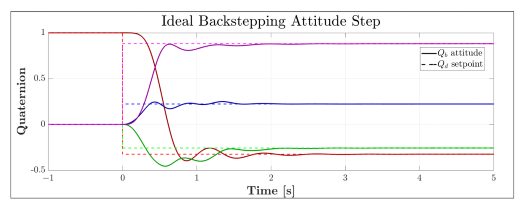
\includegraphics[width=0.7\textwidth]{graphs/IBC_Step}
\vspace{-6pt}
\caption{Quaternion attitude step}
\label{fig:IBC_Step}
\end{subfigure}
\begin{subfigure}{0.49\textwidth}
\centering
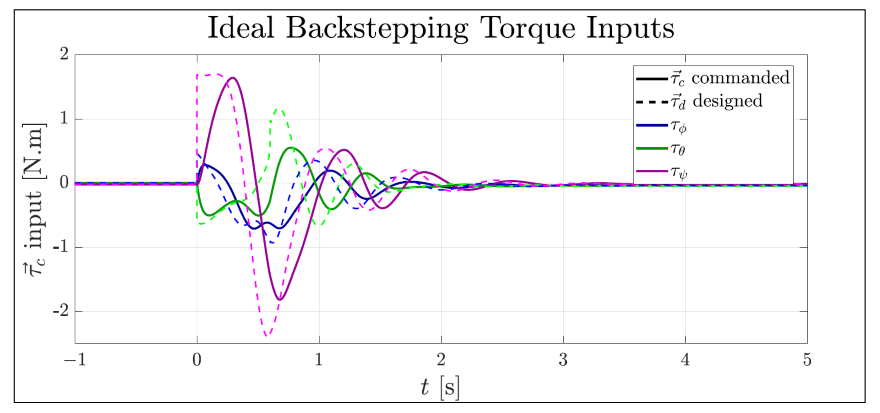
\includegraphics[width=\textwidth]{graphs/IBC_Torque}
\vspace{-20pt}
\caption{Plant input torques}
\label{fig:IBC_Torque}
\end{subfigure}
\begin{subfigure}{0.49\textwidth}
\centering
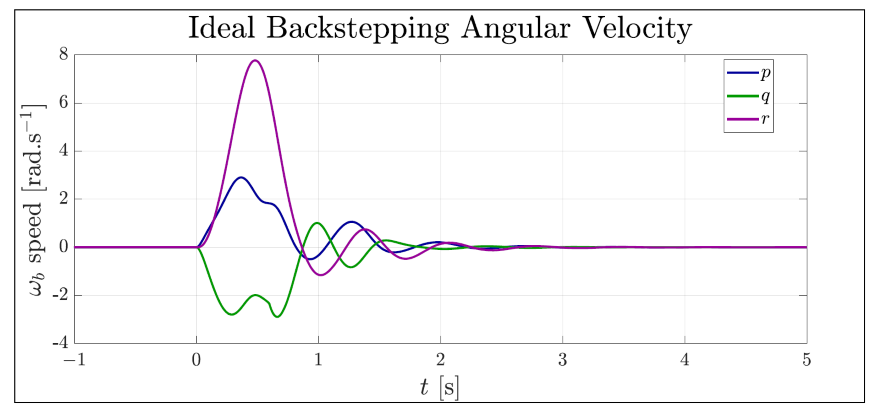
\includegraphics[width=\textwidth]{graphs/IBC_Angular}
\vspace{-20pt}
\caption{Angular velocity}
\label{fig:IBC_Angular}
\end{subfigure}
\begin{subfigure}{\textwidth}
\centering
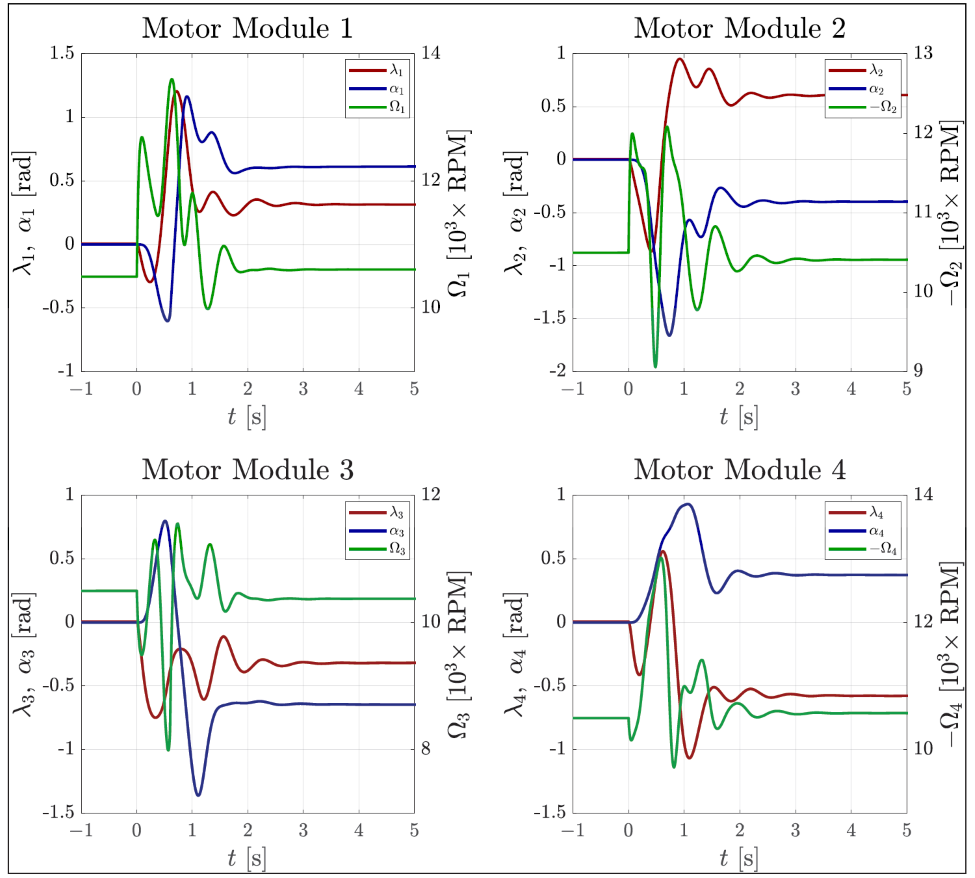
\includegraphics[width=0.6\textwidth]{graphs/IBC_Input}
\vspace{-8pt}
\caption{Plant actuator inputs}
\label{fig:IBC_Input}
\end{subfigure}
\vspace{-8pt}
\caption{Ideal backstepping controller}
\label{fig:IBC_controller_result}
\vspace{-10pt}
\end{figure}
\par
The attitude's step response in Fig:\ref{fig:IBC_Step} shows a faster response with notable oscillations introduced at the settling point. The step settles in $t_{95}=1.6403~\text{s}$, almost twice as fast as a basic PD controller. The oscillations produced at the settling point are as a result of the actuator commands (Fig:\ref{fig:IBC_Input}) reaching their rate limits, seen as a large difference between the commanded and physically actuated torque inputs in Fig:\ref{fig:IBC_Torque}. Furthermore, the commanded angular velocity changes for the IBC controller are, on average, twice that of the previous control laws which then results in increased nonlinear torque responses.
\par
The Ideal Backstepping controller is by far the most aggressive control law, which leads to sizable and perhaps unsatisfactory overshoot. That aggression is due to the exact dynamic compensation applied by the attitude control and \emph{not the applied controller gain} as is the case with the previous symmetric PD controller. Saturated rate limits of the actuators then prevent the commanded input being met by the actuated control torque. The Adaptive backstepping controller is tested and discussed later in Sec:\ref{subsec:simulation.disturbance.torque} in the context of robust trajectory stability, rather than stepped controller performances here.
%====================================================
\section{Position Controllers}
\label{sec:simulation.position}
%====================================================
Following the attitude controller optimization, a similar approach is applied to the two proposed position control laws (in Sec:\ref{sec:control.position}). It is important to specify that, for position controller optimization, a plant dependent diagonal PD attitude controller (Sec:\ref{subsubsec:simulation.atttiude.pd.dependent}) is used to stabilize the coupled attitude dynamics. To test each particle's controller coefficient performance, the attitude setpoint was kept at a constant $Q_d=[+1~\vec{0}\hspace{2pt}]^T$, while various position setpoints are applied. The same basic pseudo inversion allocator (Sec:\ref{subsec:allocation.allocators.inverse}) is used for position control to distrubte the virtual control input $\vec{\nu}_d$. Each position setpoint is defined in the inertial frame:
\begin{equation}
\vec{\mathcal{E}}_d(t)\triangleq\begin{bmatrix}
X_d(t)&
Y_d(t)&
Z_d(t)
\end{bmatrix}^T
~~~~\in\mathcal{F}^{I}
\end{equation}
A collection of position setpoints are tested, where each setpoint is positioned on the surface of a sphere at a radius of $C=5~[\text{m}]$ from a central starting point. That starting position is consistently tested at $\vec{\mathcal{E}}_0=[5~5~5]^{T}~[\text{m}]$, relative to the inertial frame's origin. Each setpoint is then stepped away from $\vec{\mathcal{E}}_0$ as per a rotated radial arm:
\begin{equation}
\vec{\mathcal{E}}_d(t)=\vec{\mathcal{E}}_0+R_y(\theta_{y})R_x(\phi_{x})\begin{bmatrix}
0 & 0 & 5
\end{bmatrix}^T
\end{equation}
Test angles $\phi_x$ and $\theta_y$ rotate the radial arm  $C$ for a range $\phi_x\in[-180\text{\textdegree}:180\text{\textdegree}]$ and $\theta_y\in[-90\text{\textdegree}:90\text{\textdegree}]$; both at $30~\text{\textdegree}$ increments. That results in test space position surface illustrated in Fig:\ref{fig:position-setpoint}, with a total of 91 position setpoints to test. Performance of each position step isevaluated with another ITAE integral for the position and translational velocity errors, both transformed into the \emph{body frame}, $\mathcal{F}^{b}$. 
\begin{equation}\label{eq:position-performance}
\vec{\zeta}_{\mathcal{E}}=\int_{t=0}^{15}C_{X}*t*||\vec{X}_e(t)||.dt+\int_{t=0}^{15}C_{v}*t*|\vec{v}_e(t)|.dt
\end{equation}
As with the attitude steps, each position steps simulation is given $t=15~\text{s}$ to reach its settling point when stepped from the starting point. Weighting coefficients $C_X$ and $C_v$ prioritize position and velocity errors respectively, both are weighted at unity. Each particle is then stepped 91 times for position ranges described above, the resultant cost of Eq:\ref{eq:position-performance} is averaged for an overall performance metric. Only plant dependent compensating position controllers are considered and optimized for the position control loop.
\par
Not compensating for the gravitational force acceleration applied to the vehicle in its differential equation of motion, Eq:\ref{eq:quaternion-states-acceleration}, \emph{would} result in instability. An uncompensated gravitational force of $15.45~[\text{N}]$ would drive both Lyapunov function derivatives, Eq:\ref{eq:position-pd-stability} for PD control and Eq:\ref{eq:4.109c} for backstepping control, away from stabilizing negative definite conditions. 
\par
To compare the relative performance of each optimized position controller, a constant position step test is applied in both cases:
\begin{equation}\label{eq:position-step}
\vec{\mathcal{E}}_d=\begin{bmatrix}
X_d&
Y_d&
Z_d
\end{bmatrix}^T=\begin{bmatrix}
7.5&
4&
3
\end{bmatrix}^T~~\text{m},~\in\mathcal{F}^{I}
\end{equation}
\par
\begin{figure}[htbp]
\vspace{-16pt}
\centering
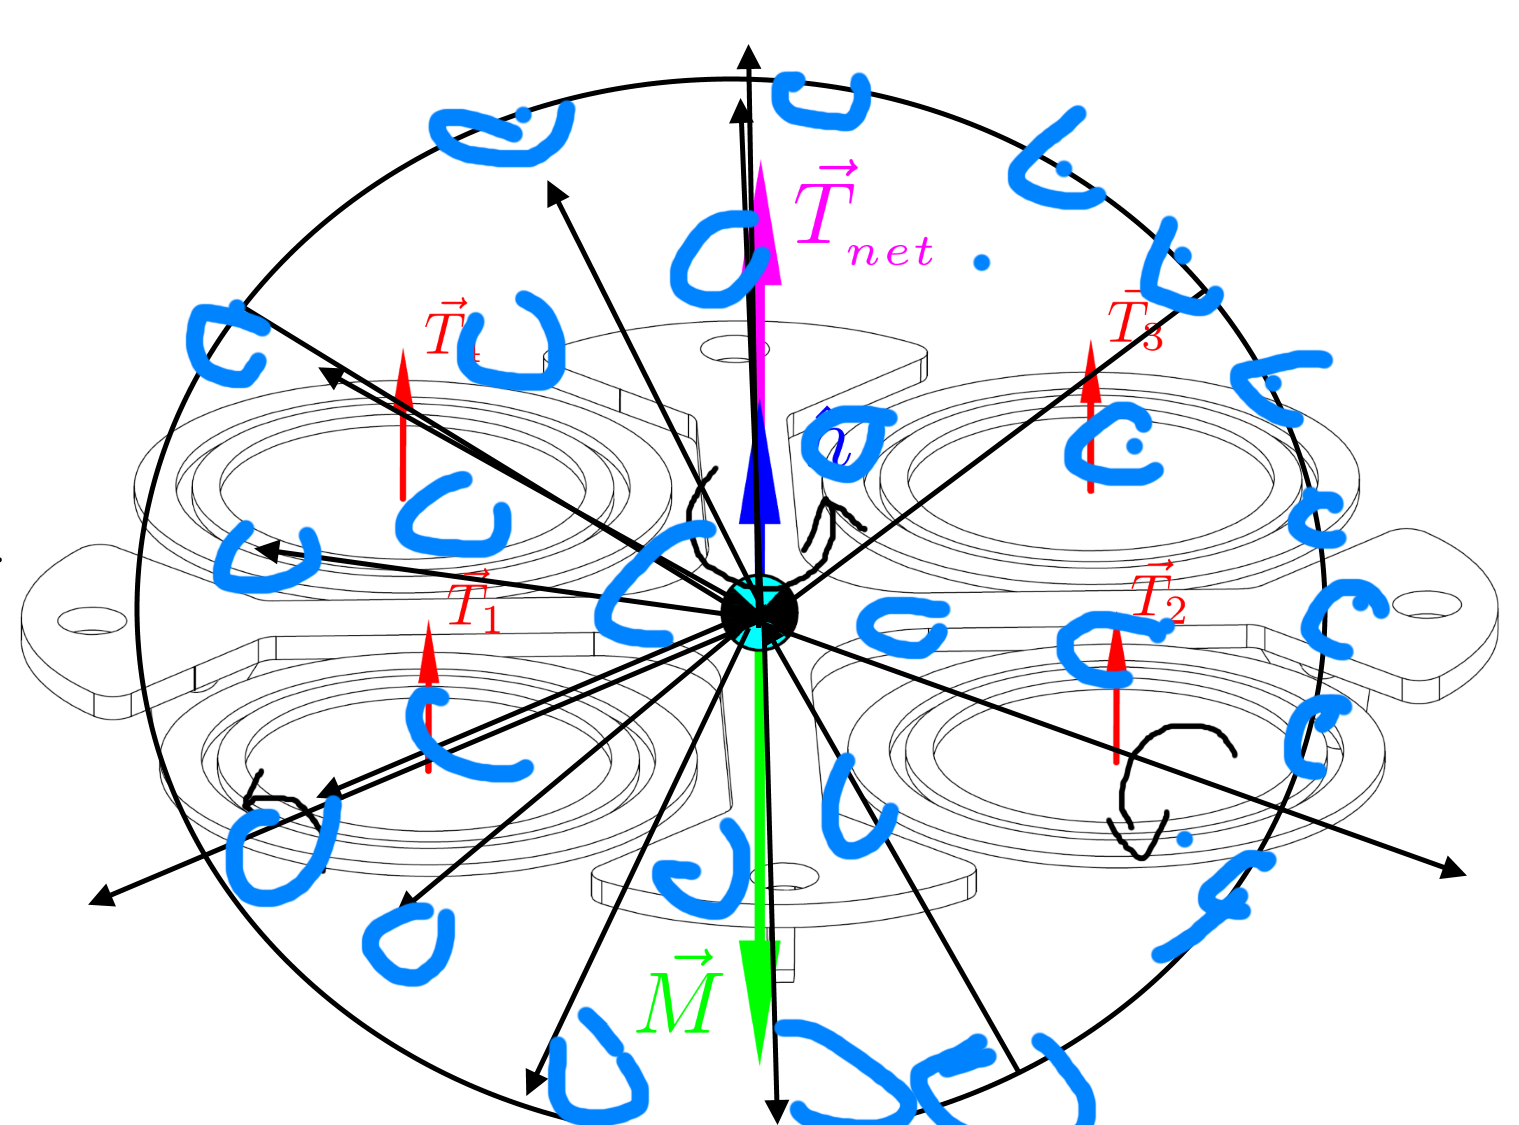
\includegraphics[width=0.72\textwidth]{figs/position-setpoint}
\vspace{-6pt}
\caption{Position setpoint workspace}
\label{fig:position-setpoint}
\vspace{-16pt}
\end{figure}
%====================================================
\subsection{PD}
\label{subsec:simulation.position.pd}
%====================================================
The reference case for position control is the Proportional-Derivative controller, presented in Sec:\ref{subsec:control.position.pd}. The PD position controller designs a control force input, from Eq:\ref{eq:position-pd}:
\begin{equation}\label{eq:optimized-position}
\vec{F}_{_{PD}}=K_p\vec{X}_e + K_d\vec{v}_e + \hat{\omega}_b\times m_b\hat{v}_b-m_b\vec{G}_b~~~~\in\mathcal{F}^{b}
\end{equation}
where $\vec{X}_e$ is the inertial position error $\vec{\mathcal{E}}_e\in\mathcal{F}^{I}$, transformed to the body frame in Eq:\ref{eq:4.80a}. Both $K_p$ and $K_d$ are diagonal gain coefficient matrices. Introducing of symmetric $[3\times 3]$ coefficients to the gain matrices did not yield any improvements for the attitude plant in Sec:\ref{subsubsec:simulation.atttiude.pd.3x3}, so it is not investigated in the context of position control. The two gain coefficients for the PD controller are structured as follows:
\begin{equation}\label{eq:simulation-attitde-pd-diagonal-coefficients}
K_p\triangleq \begin{bmatrix}
K_p(1) & 0 & 0\\
0 & K_p(2) & 0\\
0 & 0 & K_p(3)
\end{bmatrix}
~~\text{and}~~K_d\triangleq \begin{bmatrix}
K_d(1) & 0 & 0\\
0 & K_d(2) & 0\\
0 & 0 & K_d(3)
\end{bmatrix}
\end{equation}
Each coefficient matrix acts on the position error vector, $\vec{X}_e$, and the velocity error vector, $\vec{v}_e$, independently. The following coefficients are the result of the optimization process:
\begin{equation}\label{eq:optimized-position-pd}
K_p = \begin{bmatrix}
2.4167 & 0 & 0\\
0 & 2.1557 & 0\\
0 & 0 & 2.5904
\end{bmatrix}
~~\text{and}~~K_d = \begin{bmatrix}
3.4794 & 0 & 0\\
0 & 3.3846 & 0\\
0 & 0 & 3.8698
\end{bmatrix}
\end{equation}
A step in the position loop's setpoint produces a response shown in Fig:\ref{fig:PD_Position_Step}. Stepping from the initial position to the setpoint $\vec{\mathcal{E}}_d$ described in Eq:\ref{eq:attitude-step-position}. The position step settled in $t_{95}=4.007~\text{s}$ without any overshoot. 
\\
\emph{\color{Gray}Note that $\vec{\mathcal{E}}_d$ in Eq:\ref{eq:attitude-step-position} is defined in the inertial frame, $\mathcal{F}^{I}$. That setpoint is transformed to the body frame as a variable substitution for $\vec{X}_d$ for the controller error in Eq:\ref{eq:optimized-position}.}
\par
Not shown, but still considered, is the effect a position step has on the attitude plant's stability, which still remained stable at the origin with no deviations. Because the attitude setpoint is $Q_d=[+1~\vec{0}\hspace{2pt}]^T$, almost all the force requirement in steady state is to oppose the gravitational downward force acting on the body, Fig:\ref{fig:PD_Position_Force}.
\begin{figure}[htbp]
\vspace{-10pt}
\centering
\begin{subfigure}{\textwidth}
\centering
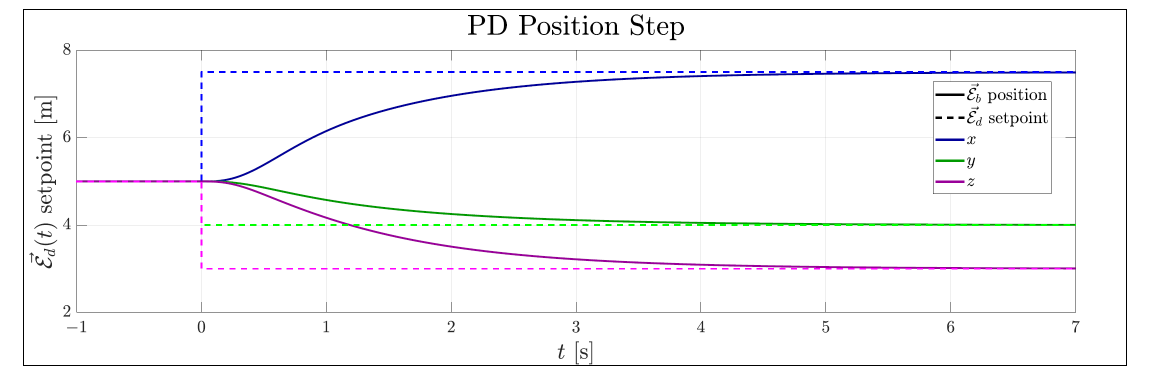
\includegraphics[width=0.7\textwidth]{graphs/PD_Position_Step}
\vspace{-6pt}
\caption{Position step}
\label{fig:PD_Position_Step}
\end{subfigure}
\begin{subfigure}{0.49\textwidth}
\centering
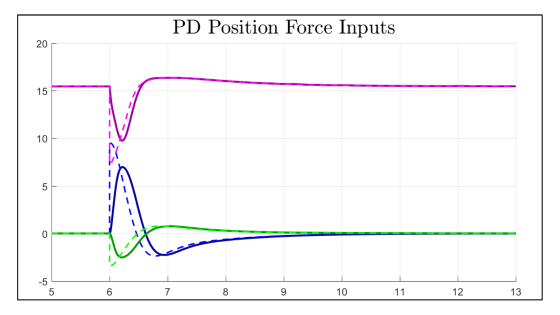
\includegraphics[width=\textwidth]{graphs/PD_Position_Force}
\vspace{-20pt}
\caption{Plant input forces}
\label{fig:PD_Position_Force}
\end{subfigure}
\begin{subfigure}{0.49\textwidth}
\centering
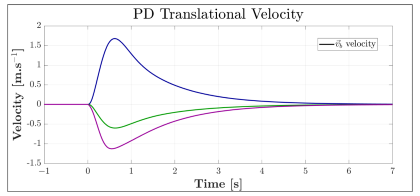
\includegraphics[width=\textwidth]{graphs/PD_Position_Velocity}
\vspace{-20pt}
\caption{Translational velocity}
\label{fig:PD_Position_Velocity}
\end{subfigure}
\begin{subfigure}{\textwidth}
\centering
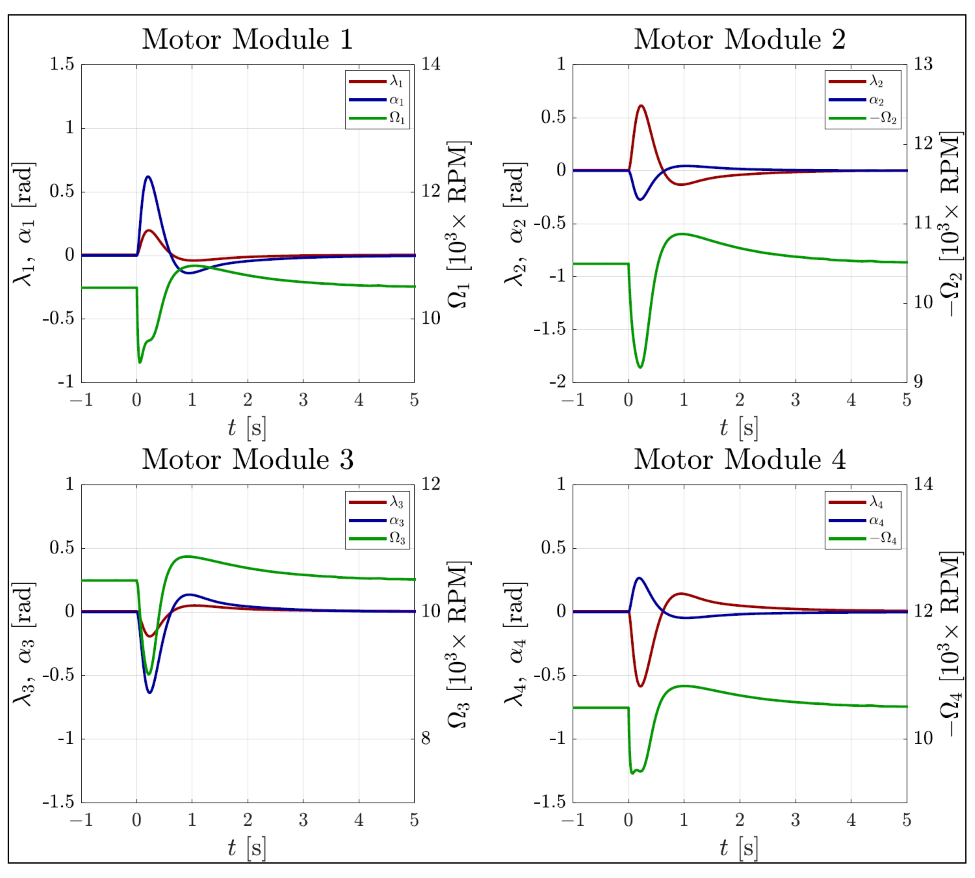
\includegraphics[width=0.6\textwidth]{graphs/PD_Position_Input}
\vspace{-8pt}
\caption{Plant actuator inputs}
\label{fig:PD_Position_Input}
\end{subfigure}
\vspace{-8pt}
\caption{Position PD}
\vspace{-34pt}
\end{figure}
%====================================================
\subsection{Ideal and Adaptive Position Backstepping}
\label{subsec:simulation.position.pd}
%====================================================
The second and final position controller to be tested is the Ideal Backstabbing controller, the only exponentially stable position control law reviewed. As is the case with attitude IBC, the coefficients selected for the Ideal Backstepping case are used again for the Adaptive case, the latter is evaluated subsequently in Sec:\ref{subsec:simulation.disturbance.force}. Recalling the position IBC structure from Sec:\ref{subsec:control.position.bacstepping}:
\begin{equation}\label{eq:simulation-position-IBC}
\vec{F}_{_{IBC}}=m_b\Big(\big(1+\Gamma_1\Gamma_2\big)\vec{\zeta}_1-\big(\Gamma_1+\Gamma_2\big)\hat{v}_b\big)\Big)+\hat{\omega}_b\times m_b\hat{v}_b-m_b\vec{G}_b~~~~\in\mathcal{F}^{b}
\end{equation}
with the backstepping variable $\vec{\zeta}_1$ defined $\vec{z}_1\triangleq \vec{X}_e$, from Eq:\ref{eq:102a}. 
\par
The two positive symmetric coefficient gain matrices in Eq:\ref{eq:simulation-position-IBC} are structured as:
\begin{equation}\label{eq:simulation-position-diagonal-coefficients}
\Gamma_1\triangleq \begin{bmatrix}
\Gamma_1(1) & \Gamma_1(4) & \Gamma_1(5)\\
\Gamma_1(4) & \Gamma_1(2) & \Gamma_1(6)\\
\Gamma_1(5) & \Gamma_1(6) & \Gamma_1(3)
\end{bmatrix}
~~\text{and}~~\Gamma_2\triangleq \begin{bmatrix}
\Gamma_2(1) & \Gamma_2(4) & \Gamma_2(5)\\
\Gamma_2(4) & \Gamma_2(2) & \Gamma_2(6)\\
\Gamma_2(5) & \Gamma_2(6) & \Gamma_2(3)
\end{bmatrix}
\end{equation}
Similar to the attitude backstepping controller, the position ideal backstepping controller has gain coefficients which act on both plant's error $\vec{X}_e$ and error rates $\vec{v}_e$. This makes local and global coefficient position selection difficult without adversely affecting the swarm's optimization trajectory process. Using the first coefficient matrix $\Gamma_1$ to prioritize position tracking errors $\vec{X}_e$ and relegating $\Gamma_2$ to settle velocity errors $\vec{v}_e$, the local best positions are chosen where each respective error is minimized. The optimized gain coefficients for $\Gamma_1$ and $\Gamma_2$ were then produced by the PSO algorithm:
\begin{equation}\label{eq:optimized-Position-IBC}
\Gamma_1 = \begin{bmatrix*}
2.3409 & 0.1707 & -0.1644\\
0.1707 & 2.0493 & 0.1060\\
-0.1644 & 0.1060 & 1.7322
\end{bmatrix*}
~~\text{and}~~\Gamma_2= \begin{bmatrix*}
1.5287 & 0.02928 & 0.0816\\
0.0292 & 1.4214 & -0.0410\\
0.0816 & -0.0410 & 1.4753
\end{bmatrix*}
\end{equation}
\begin{figure}[htbp]
\vspace{-20pt}
\centering
\begin{subfigure}{\textwidth}
\centering
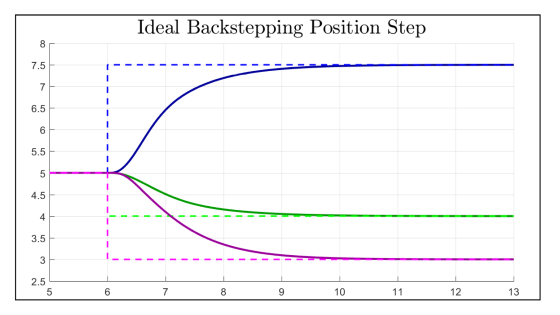
\includegraphics[width=0.7\textwidth]{graphs/IBC_Position_Step}
\vspace{-6pt}
\caption{Position step}
\label{fig:IBC_Position_Step}
\end{subfigure}
\begin{subfigure}{0.49\textwidth}
\centering
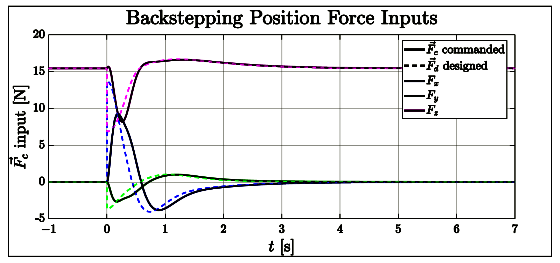
\includegraphics[width=\textwidth]{graphs/IBC_Position_Force}
\vspace{-20pt}
\caption{Plant input forces}
\label{fig:IBC_Position_Force}
\end{subfigure}
\begin{subfigure}{0.49\textwidth}
\centering
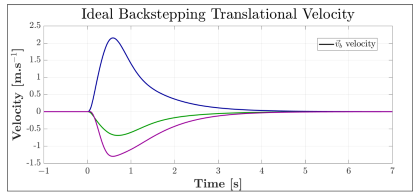
\includegraphics[width=\textwidth]{graphs/IBC_Position_Velocity}
\vspace{-20pt}
\caption{Translational velocity}
\label{fig:IBC_Position_Velocity}
\end{subfigure}
\begin{subfigure}{\textwidth}
\centering
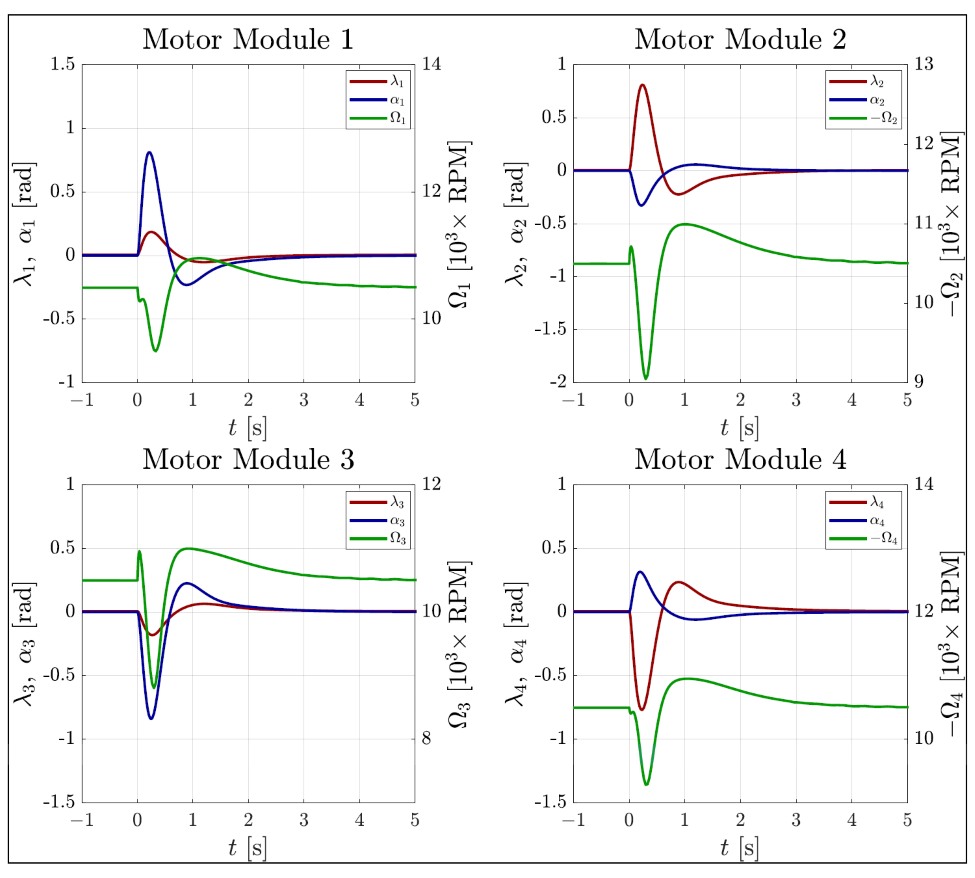
\includegraphics[width=0.6\textwidth]{graphs/IBC_Position_Input}
\vspace{-8pt}
\caption{Plant actuator inputs}
\label{fig:IBC_Position_Input}
\end{subfigure}
\vspace{-8pt}
\caption{Position backstepping controller}
\vspace{-20pt}
\end{figure}
\par
Fig:\ref{fig:IBC_Position_Step} shows how the Ideal Backstepping controller stabilizes and tracks a step change to the translational position setpoint. Note that the position plotted in Fig:\ref{fig:IBC_Position_Step} is the relative position in the inertial frame $\mathcal{F}^{I}$, not the backstepping input $\vec{X}_e\in\mathcal{F}^b$. The Ideal Backstepping controller settles in $t_{95}=2.987~[\text{s}]$, faster than a regular proportional-derivative position controller. The exponentially bound error trajectory improves the controller's performance but, not unexpectedly, commands greater input forces (Fig:\ref{fig:IBC_Position_Force}) from larger spikes in the propeller's rotational speed, shown in Fig:\ref{fig:IBC_Input}. 
\par
The improved performance from the position Ideal Backstepping controller is due to the change in structure, increasing the PD controller's gain by a scale factor of 2 (analogous to the test performed in Fig:\ref{fig:PD_Diagonal_Gain_Step}) \emph{decreases} the step's settling time from $t_{95}=4.007~[\text{s}]$ to $4.379~[\text{s}]$. So improving even the conceptually simpler force position control loop is not as easy as simply adding more gain to the control plant. 
\begin{figure}[htbp]
\vspace{-12pt}
\centering
\begin{subfigure}{\textwidth}
\centering
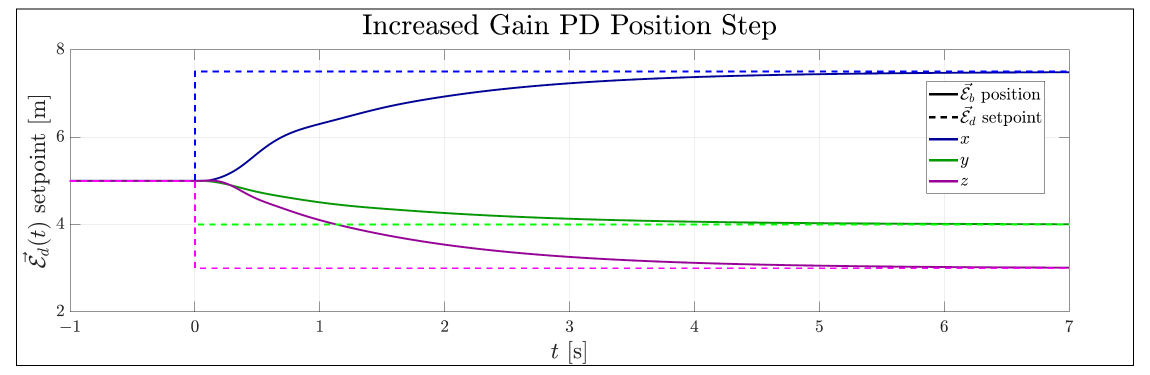
\includegraphics[width=0.7\textwidth]{graphs/PD_Position_Gain_Step}
\vspace{-6pt}
\caption{Position step}
\label{fig:PD_Position_Gain_Step}
\end{subfigure}
\begin{subfigure}{\textwidth}
\vspace{-4pt}
\centering
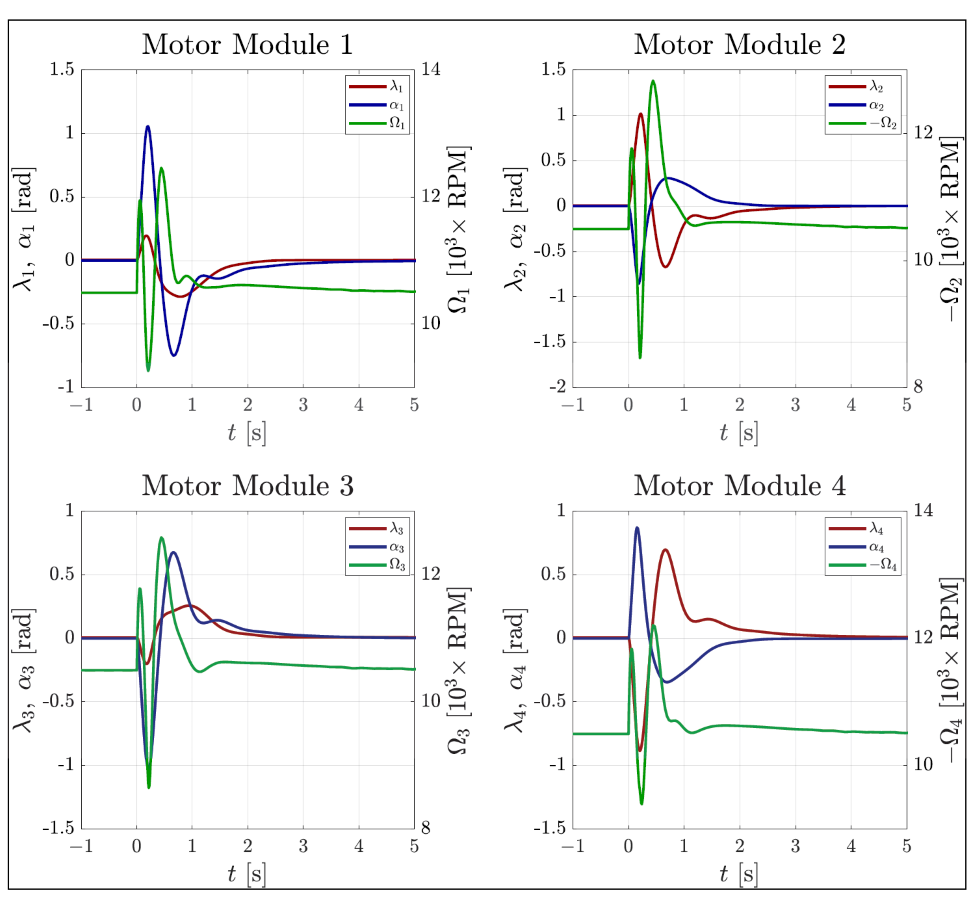
\includegraphics[width=0.59\textwidth]{graphs/PD_Position_Gain_Input}
\vspace{-8pt}
\caption{Plant actuator inputs}
\label{fig:PD_Position_Gain_Input}
\end{subfigure}
\vspace{-8pt}
\caption{Increased gain PD position}
\vspace{-36pt}
\end{figure}
%====================================================
\section{Setpoint Control Results}
\label{sec:simulation.autopilot}
%====================================================
None of the proposed attitude or position controllers are unstable, each one achieves the goal of setpoint tracking in the context of stepped inputs. To corroborate dynamic setpoint tracking an increasing (\emph{chirp}) trajectory is commanded, illustrated in Fig:\ref{fig:trajectory}. The trajectory applies an increasing frequency rate of $1/60~[\text{Hz}.s^{-1}]$ starting from zero, such that at $t=60~[\text{s}]$ the trajectory orbits a central point $\vec{C}_0$ and completes a single orbit every minute. Eventually the increasing orbital frequency will push each controller beyond their tracking limit. Only two Proportional Derivative \emph{attitude} controllers are tested here, both with diagonal gain matrices (from Eq:\ref{eq:optimized-pd-independent}), to compare the effects of plant dependent compensation. It was shown previously that symmetric gain coefficients yield no performance improvements for the PD case, so only diagonal coefficient matrices were used. 
\par
Furthermore, Sec:\ref{subsec:simulation.attitude.pd} demonstrated plant independent controllers result in steady state errors, the same is shown to be true for trajectory tracking. Adaptive backstepping controllers and their disturbance rejection properties are only discussed next in Sec:\ref{sec:simulation.disturbance}. Each attitude controller is tested together with a common PD position controller, tracking the orbital XYZ position. Similarly each position controller is tested using a simple diagonal PD controller to track the attitude. The attitude controllers have an initial step to reach the orbital attitude from their starting attitude, $Q_0=[+1~\vec{0}\hspace{2pt}]^T$. Each controller's trajectory setpoint response and its respective tracking error are plotted together in pairs.
\begin{figure}[htbp]
\centering
\vspace{-10pt}
\begin{subfigure}{0.9\textwidth}
\centering
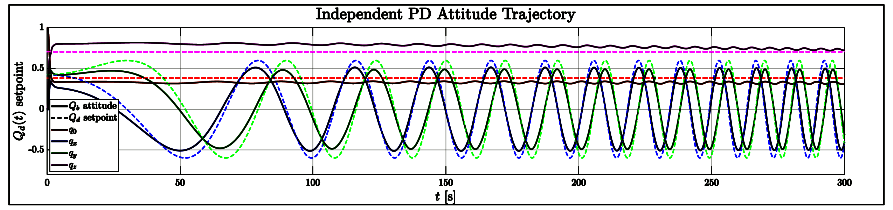
\includegraphics[width=\textwidth]{graphs/PD_Diagonal_Independent_Trajectory}
\vspace{-18pt}
\caption{Attitude trajectory}
\label{fig:independent_diagonal_trajectory}
\end{subfigure}
\begin{subfigure}{0.9\textwidth}
\centering
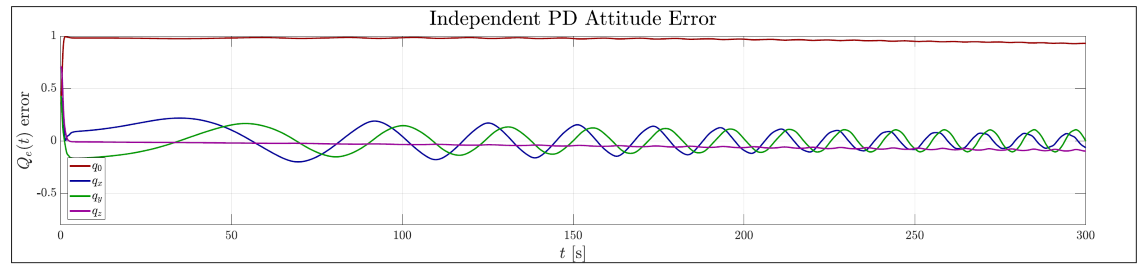
\includegraphics[width=\textwidth]{graphs/PD_Diagonal_Independent_Error}
\vspace{-18pt}
\caption{Attitude trajectory error}
\label{fig:independent_diagonal_error}
\end{subfigure}
\vspace{-10pt}
\caption{Independent PD attitude controller}
\label{fig:independent}
\end{figure}
\begin{figure}[htbp]
\centering
\vspace{-20pt}
\begin{subfigure}{0.9\textwidth}
\centering
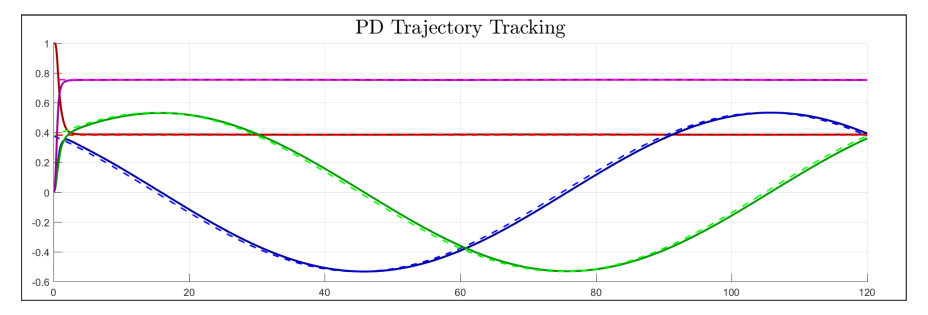
\includegraphics[width=\textwidth]{graphs/PD_Diagonal_Dependent_Trajectory}
\vspace{-18pt}
\caption{Attitude trajectory}
\label{fig:dependent_diagonal_trajectory}
\end{subfigure}
\begin{subfigure}{0.9\textwidth}
\centering
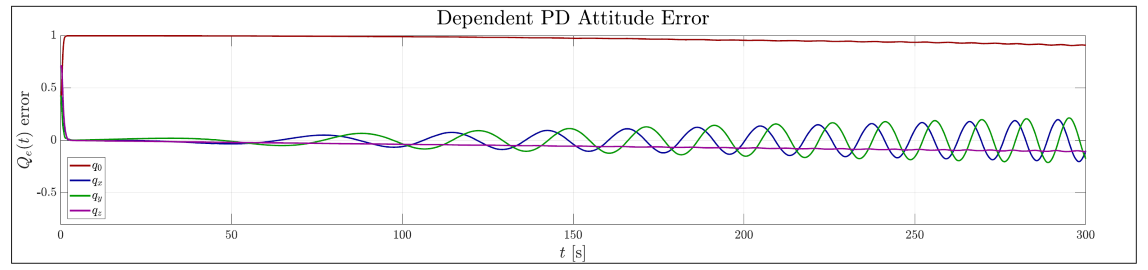
\includegraphics[width=\textwidth]{graphs/PD_Diagonal_Dependent_Error}
\vspace{-18pt}
\caption{Attitude trajectory error}
\label{fig:dependent_diagonal_error}
\end{subfigure}
\vspace{-10pt}
\caption{Dependent PD attitude controller}
\label{fig:dependent}
\end{figure}
\begin{figure}[hbtp]
\centering
\vspace{-20pt}
\begin{subfigure}{0.9\textwidth}
\centering
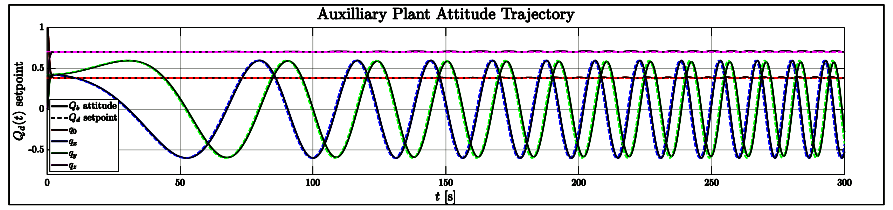
\includegraphics[width=\textwidth]{graphs/XPD_Trajectory}
\vspace{-18pt}
\caption{Attitude trajectory}
\label{fig:XPD_trajectory}
\end{subfigure}
\vspace{-32pt}
\end{figure}
\newpage
\begin{figure}[htbp]
\centering
\ContinuedFloat
\begin{subfigure}{0.9\textwidth}
\centering
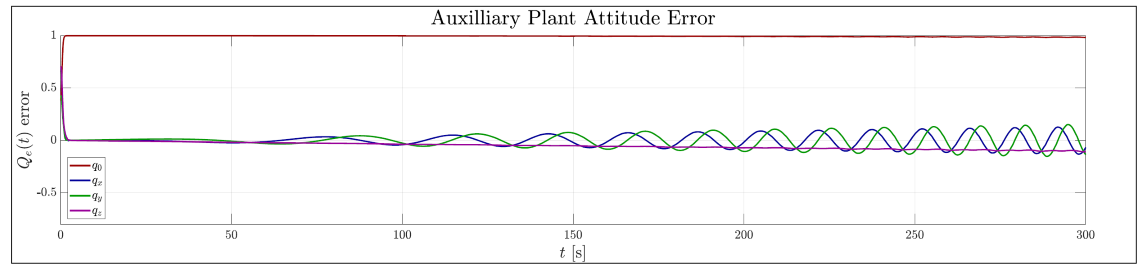
\includegraphics[width=\textwidth]{graphs/XPD_Error}
\vspace{-18pt}
\caption{Attitude trajectory error}
\label{fig:dependent_diagonal_error}
\end{subfigure}
\vspace{-10pt}
\caption{Auxiliary PD attitude controller}
\label{fig:auxiliary}
\end{figure}
\begin{figure}[htbp]
\centering
\vspace{-8pt}
\begin{subfigure}{0.9\textwidth}
\centering
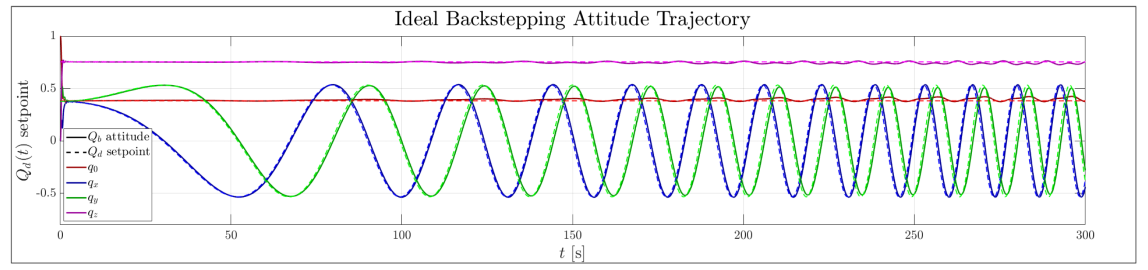
\includegraphics[width=\textwidth]{graphs/IBC_Trajectory}
\vspace{-18pt}
\caption{Attitude trajectory}
\label{fig:backstepping_trajectory}
\end{subfigure}
\begin{subfigure}{0.9\textwidth}
\centering
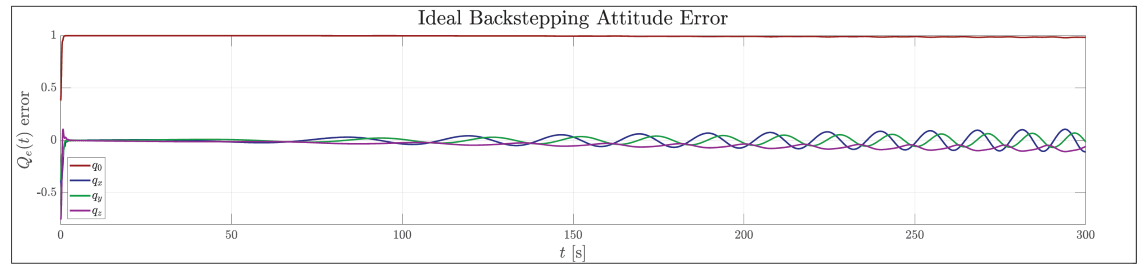
\includegraphics[width=\textwidth]{graphs/IBC_Error}
\vspace{-18pt}
\caption{Attitude trajectory error}
\label{fig:backstepping_error}
\end{subfigure}
\vspace{-10pt}
\caption{Ideal backstepping attitude controller}
\label{fig:backstepping}
\end{figure}
Interestingly, even the uncompensated (still compensating for gravitational force however) controller can still track the generated trajectory. The independent PD controller, illustrated in Fig:\ref{fig:independent}, has a \emph{roughly} constant quaternion error which oscillates with the trajectory setpoint. Only beyond an orbital rate of $\approx 1~[\text{Hz}]$, at $t=60~[\text{s}]$, does the trajectory begin to lose its stability, where the quaternion errors start to drift. Introducing plant compensation in Fig:\ref{fig:dependent} reduces the trajectory's initial error. The plant dependent PD controller begins to show oscillatory tracking errors at the same $\approx 1~[\text{Hz}]$ point and slowly drifts from its setpoint.
\par
The exponentially stable controllers performed better and maintained approximately zero error trajectory tracking for longer. The auxiliary PD controller, Fig:\ref{fig:auxiliary}, starts to introduce a non-zero oscillatory tracking error at a greater $\approx 1.4~[\text{Hz}]$, at $t=70~[\text{s}]$. The auxiliary PD controller still maintains an acceptable error ($<5\%$) until a trajectory rate of $\approx 3.5~[\text{Hz}]$ is reached at $t=110~[\text{s}]$. The final, ideal backstepping controller in Fig:\ref{fig:backstepping} retains an error free trajectory for the longest, only introducing oscillating tracking errors at $\approx 1.8~[\text{Hz}]$, at $t=80~[\text{s}]$, but continues tracking the trajectory with an acceptable ($<5\%$) error up to an orbital rate of $\approx 5.4~[\text{Hz}]$ until $t=140~[\text{s}]$. Trajectory errors could be reduced (\emph{improved}) further with the application of higher order state derivative trajectory setpoints for each controller with $\vec{\omega}_d\not=\vec{0}$ and $\vec{v}_d\not=\vec{0}$).
\newpage
\begin{figure}[htbp]
\centering
\vspace{-8pt}
\begin{subfigure}{0.9\textwidth}
\centering
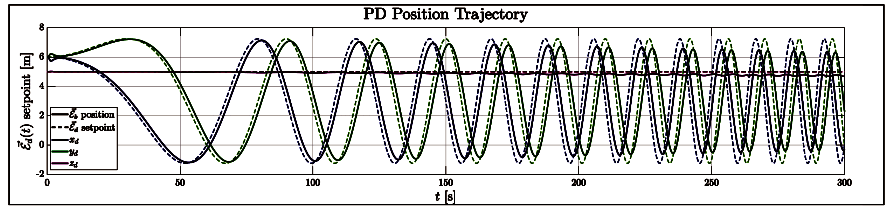
\includegraphics[width=\textwidth]{graphs/PD_Position_Trajectory}
\vspace{-18pt}
\caption{Position trajectory}
\label{fig:pd_position_trajectory}
\end{subfigure}
\begin{subfigure}{0.9\textwidth}
\centering
\includegraphics[width=\textwidth]{graphs/PD_Position_Error}
\vspace{-18pt}
\caption{Position trajectory error}
\label{fig:pd_position_error}
\end{subfigure}
\vspace{-10pt}
\caption{PD position controller}
\label{fig:pd_position}
\end{figure}
\begin{figure}[htbp]
\centering
\vspace{-8pt}
\begin{subfigure}{0.9\textwidth}
\centering
\includegraphics[width=\textwidth]{graphs/IBC_Position_Trajectory}
\vspace{-18pt}
\caption{Position trajectory}
\label{fig:ibc_position_trajectory}
\end{subfigure}
\begin{subfigure}{0.9\textwidth}
\centering
\includegraphics[width=\textwidth]{graphs/IBC_Position_Error}
\vspace{-18pt}
\caption{Position trajectory error}
\label{fig:ibc_position_error}
\end{subfigure}
\vspace{-10pt}
\caption{Backstepping position controller}
\label{fig:ibc_position}
\end{figure}
Ideal backstepping and PD position controllers manifest a small lag behind the generated XYZ position trajectorys. This is a consequence of tracking only first order setpoints, if a velocity setpoint was applied as well that tracking error would be diminished. Both controllers track the trajectory setpoint with a non-zero error from the start of the simulation. The ideal backstepping position controller does, however, track increasingly faster trajectories with a smaller error, shown in Fig:\ref{fig:ibc_position_error}.
%====================================================
\section{Robust Stability and Disturbance Rejection}
\label{sec:simulation.disturbance}
%====================================================
Despite deriving adaptive control laws in Sec:\ref{subsubsec:control.attitude.nonlinear.adaptivebackstep} and Sec:\ref{subsec:control.position.bacstepping} for attitude and position controllers respectively, each of the proposed control law demonstrated acceptable stability under sizable disturbances. Trajectories tested under distrubance conditions are simple oscillatory ones, similar to the trajectory setpoint illustrated in Fig:\ref{fig:trajectory} but with a \emph{constant} orbital rate of $0.5~[\text{Hz}]$ applied. The purpose of the subsequent tests is to evaluate the disturbance approximator's performance, not a particular controller's trajectory tracking ability. App:\ref{app:disturbance} shows each non-adaptive controller's trajectory response to uncompensated disturbances acting on the vehicle.
%====================================================
\subsection{Torque Disturbance Rejection}
\label{subsec:simulation.disturbance.torque}
%====================================================
Torque turbulences are difficult to define without in-depth accompanying statistical and mathematical analysis. To expedite the stability/disturbance evaluation process, torque turbulences were approximated using a Dryden Gust model,\cite{optimalgust,discretegustmodel}. That gust/wind turbulence model is designed for helicopters in hovering conditions, but the propeller span dimension was scaled accordingly. Alternatively the Von Karman aerospace disturbance model(s) could be implemented but that model is computationally more exhaustive. The accuracy of the turbulence model is not particularly important given that this section aims to evaluate the adaptive backstepping observer's performance at estimating a \emph{general} disturbance. Consideration of more applicable wind and disturbance models similar to \cite{nonlineardynamics} remains open to further research.
\par
Without deliberating on the details of the model, in short the Dryden Wind model produces turbulence signals from white noise filtered through a specified power spectrum. That power spectrum varies as per an aircraft's orientation, altitude and translational velocity. For the aircraft and trajectory under consideration here such a disturbance model is sufficient for simulating small interference patterns. Recall the torque disturbance observer derived for the attitude backstepping plant, from Eq:\ref{eq:asymptotic-disturbance}:
\begin{equation}\label{eq:stability-torque-overserver}
\dot{\hat{\tau}}_L=-\Gamma_L J_b^{-1}(u)\big(\Gamma_1\vec{q}_e-\hat{\omega_b}\big)
\end{equation}
The gain adaptivity matrix $\Gamma_L$ is tuned using a PSO iteration loop, simulated in steady state with a cost function to minimize the observer's error $\Delta\hat{\tau}_L$ over the course of a $t=60~[\text{s}]$ simulation. The resultant \emph{diagonal} $[3\times 3]$ adaptivity matrix is $\Gamma_L=diag(29.58,~28.43,~4.60)$. The approximator tracks an applied disturbance as shown in Fig:\ref{fig:torque-observer} over a disturbance range of $\pm 0.2~\text{N.m}$, 20\% of a typical controller's commanded input for a stepped attitude from Eq:\ref{eq:attitude-step-position}, for a short steady state test. Both pitch $\phi$ and roll $\theta$ torque approximator channels track the torque with a relatively small error, averaged $16\%$ and $15\%$ respectively. Greater deviation from the applied torque occurs in the $\psi$ channel about the $\hat{Z}_b$ axis, approximate $36\%$ averaged over the short steady state.
\begin{figure}[htbp]
\vspace{-10pt}
\centering
\includegraphics[width=0.8\textwidth]{graphs/torque-observer}
\vspace{-10pt}
\caption{Attitude torque disturbance observer}
\vspace{-18pt}
\label{fig:torque-observer}
\end{figure}
\par
Fig:\ref{fig:ABC_trajectory} shows the Adaptive Backstepping controller's attitude response over a constant orbital trajectory whilst undergoing torque turbulence. The addition of a torque observer for compensation produces a slight improvement over an uncompensated IBC controller, included in Fig:\ref{fig:app-attitude-ibc-dist} from App:\ref{app:disturbance}. The improvement a torque observer yields is diminished given that in an Ideal Backstepping case the actuators were being rate limited (Fig:\ref{fig:IBC_Input}). Higher bandwidth torque inputs will not see much improvement given that the actuators cannot apply the commanded input at a sufficient rate.
\begin{figure}[hbtp]
\vspace{-6pt}
\centering
\includegraphics[width=0.8\textwidth]{graphs/ABC_trajectory}
\vspace{-10pt}
\caption{Adaptive backstepping attitude trajectory tracking}
\label{fig:ABC_trajectory}
\vspace{-16pt}
\end{figure}
%====================================================
\subsection{Disturbance Force Rejection}
\label{subsec:simulation.disturbance.force}
%====================================================
Force disturbances are similarly emulated in simulation using a Dryden Gust model for wind turbulent velocity generation. Additionally, a wind vector field across the inertial frame test space is also used to introduce a constant force offset throughout the trajectory simulation. The force disturbance observer, from Eq:\ref{eq:abc-asymptotic-position}, has an estimate update rule such that:
\begin{equation}
\dot{\hat{F}}_D=-m_b^{-1}\Gamma_D\Big(\Gamma_1\vec{X}_e-\vec{v}_b\Big)
\end{equation}
Where $\vec{X}_e$ is the inertial position error transformed to the body frame, $\vec{X}_e=Q_b\otimes\vec{\mathcal{E}}_e\otimes Q_b^*$. Then $\Gamma_D$ is the force disturbance observer's adaptivity $[3\times 3]$ gain matrix. The gain matrix is chosen to minimize the force disturbance observer's error over a steady state simulation. Using the optimized coefficients $\Gamma_D=diag(4.20,~3.84,~3.97)$ the observer tracks a force disturbance acting on the vehicle over a range of $[-4:8]~\text{N}$. Fig:\ref{fig:force-observer} shows how the force observer adapts to the variable force turbulence applied, the plot is taken over an entire simulation (until $t=120~\text{s}$) to illustrate the vector field effects. Each observer channel ($F_x$,$F_y$ and $F_z$) averaged between $5\%$ and $10\%$ error over the course of the simulation.
\begin{figure}[hbtp]
\vspace{-6pt}
\centering
\includegraphics[width=0.8\textwidth]{graphs/force-observer}
\vspace{-10pt}
\caption{Position force disturbance observer}
\label{fig:force-observer}
\vspace{-18pt}
\end{figure}
\par
The position adaptive backstepping controller then tracks the inertial frame trajectory as shown in Fig:\ref{fig:ABC_Position_Trajectory}. The trajectory tracking performance is improved marginally when compared to the Ideal backstepping case from Fig:\ref{fig:app-position-ibc-dist}. Even without adaptive disturbance compensation, the plant is stable throughout the trajectory albeit somewhat noisy. The drawback of this particular adaptive compensation approach is that each observer is an extracted signal from existing state variables, as a result no new information is being used to compensate the plant and as such the small signal stability is largely unaffected. The vector force field produces an oscillating error from the trajectory, despite the adaptive compensation applied to the control loop, shown in Fig:\ref{fig:ABC_Position_Trajectory}.
\begin{figure}[hbtp]
\vspace{-6pt}
\centering
\includegraphics[width=0.8\textwidth]{graphs/ABC_Position_Trajectory}
\vspace{-12pt}
\caption{Adaptive backstepping position trajectory tracking}
\label{fig:ABC_Position_Trajectory}
\vspace{-16pt}
\end{figure}
%====================================================
\section{Allocation Tests}
\label{sec:simulation.allocator}
%====================================================
The various allocation rules, as derived in Ch:\ref{ch:allocation}, implement virtual control inputs to solve for explicit actuator positions. Each of the allocators tested here were compared with basic position and attitude Proportional Derivative controllers commanding a virtual input. 
\par
The abstraction applied to achieve an affine relationship required for inversion allocation (in Eq:\ref{eq:allocator-test}) meant that actuator transfer rates were independent from the allocation rule applied. As a result the affect of different allocation laws is depreciated.
\begin{subequations}\label{eq:allocator-test}
\begin{equation}\label{eq:allocator-test.a}
\vec{\nu}_c=B'(\vec{\mathbf{x}},t)u=\begin{bmatrix}
\mathbb{I}_{3\times 3} & \mathbb{I}_{3\times 3} & \mathbb{I}_{3\times 3} & \mathbb{I}_{3\times 3}\\
[\vec{L}_1]_\times & [\vec{L}_2]_\times & [\vec{L}_3]_\times & [\vec{L}_4]_\times
\end{bmatrix}
\vec{T}_{[1:4]}^T
\end{equation}
\vspace{-10pt}
\begin{equation}
u_i = \begin{bmatrix}
\Omega_i & \lambda_i & \alpha_i
\end{bmatrix}^T = R^\dagger(\vec{\mathbf{x}},\vec{T}_i,t)~~\text{for}~i\in[1:4]
\end{equation}
\end{subequations}
The transfer rate at which physically commanded inputs implement virtually designed control inputs, $\vec{\nu}_c\rightarrow\vec{\nu}_d$, is affected by the thrust inversion relationship $R^\dagger(\vec{\mathbf{x}},t)$, not allocation rules $B'(\vec{\mathbf{x}},t)$. The consequence of this is that, in the context of actuator transfer rates, each allocation rule performed almost identically. Inverse solutions to Eq:\ref{eq:allocation-quadratic} solve for the quadratic least squares minimized actuator positions. That means that each $|\vec{T}_i|$  within the $\mathbb{R}^{1\times 12}$ matrix $|\vec{T}_{[1:4]}|$ is minimized. The solution is a cost efficient one minimizing actuator effort. In general psuedo inversion, weighted and priority normalized inverse allocators each stem from Eq:\ref{eq:inversion}: 
\begin{subequations}
\begin{equation}
\vec{T}_{[1:4]}
=\big(\mathbb{I}_{m\times m}-CB(\vec{\mathbf{x}},t)\big)\vec{T}_p+C\vec{\nu}_d
\end{equation}
\vspace{-10pt}
\begin{equation}\label{eq:allocation-inversion-eq}
C=W^{-1}B^T(\vec{\mathbf{x}},t)\big(B(\vec{\mathbf{x}},t)W^{-1}B^T(\vec{\mathbf{x}},t)\big)^{-1}
\end{equation}
\end{subequations}
A combined step of setpoints for attitude \emph{and} position states is used to compare each allocation rule. A pseudo inverse allocator from Eq:\ref{eq:pseudo-inversion} is used as the reference case against which subsequent allocator algorithms are evaluated. The typical setpoint used for both position and attitude steps with attitude in Euler angles, $\vec{\eta}_d$ not quaternions $Q_d$, is:
\begin{equation}\label{eq:simulation-state-step}
\vec{\mathbf{x}}_d=\begin{bmatrix}
\vec{\mathcal{E}}_d\\
\vec{\eta}_d
\end{bmatrix}
=
\begin{bmatrix}
\begin{bmatrix}
7.5 & 4 & 3
\end{bmatrix}^T\\
\begin{bmatrix}
-142 & 167 & -45
\end{bmatrix}^T
\end{bmatrix}~~~~\begin{bmatrix}
[\text{m}]\\
[\text{\textdegree}]
\end{bmatrix}
\end{equation}
A pseudo inverse allocation solves for $\vec{T}_{[1:4]}$ using $B^\ddagger(\vec{\mathbf{x}},t)\vec{\nu}_d$, from Eq:\ref{eq:pseudo-inversion}. Fig:\ref{fig:pseudo-inverse-step} shows the combined position and attitude step responses. The combined attitude and position step response with a pseudo inverse allocator $B^\ddagger(\vec{\mathbf{x}},t)$ settles for \emph{both} states in $t_{95}=5.658~\text{s}$ from the state step. The commanded actuator inputs, as per the pseudo inverse allocator, are shown in Fig:\ref{fig:pseudo_inverse_input}.
\begin{figure}[hbtp]
\centering
\begin{subfigure}{\textwidth}
\centering
\includegraphics[width=0.8\textwidth]{graphs/pseudo_inverse_attitude}
\vspace{-4pt}
\caption{Attitude Step}
\label{fig:pseudo_inverse_attitude}
\end{subfigure}
\begin{subfigure}{\textwidth}
\vspace{-3pt}
\centering
\includegraphics[width=0.8\textwidth]{graphs/pseudo_inverse_position}
\caption{Position Step}
\label{fig:pseudo_inverse_position}
\end{subfigure}
\vspace{-2pt}
\caption{Pseudo inverse step response}
\label{fig:pseudo-inverse-step}
\vspace{-12pt}
\end{figure}
\par
\begin{figure}[htbp]
\ContinuedFloat
\begin{subfigure}{\textwidth}
\centering
\includegraphics[width=0.6\textwidth]{graphs/pseudo_inverse_input}
\vspace{-6pt}
\caption{Pseudo inverse actuator commands}
\label{fig:pseudo_inverse_input}
\end{subfigure}
\vspace{-10pt}
\caption{Pseudo inverse step response}
\vspace{-16pt}
\end{figure}
The preferred allocator positions, described in Sec:\ref{subsec:allocation.allocators.norminverse}, are hovering conditions defined with respect to either the inertial or body frames, $\mathcal{F}^{I}$ and $\mathcal{F}^{b}$ respectively. At steady state with an attitude at the origin, $Q_d=[+1~\vec{0}\hspace{2pt}]^T$, the controller commands the virtual control input:
\begin{equation}\label{eq:hover-actuator}
\vec{\nu}_p=\begin{bmatrix}
\vec{F}_p\\
\vec{\tau}_p
\end{bmatrix}
=
\begin{bmatrix}
\begin{bmatrix}
0&0&15.45
\end{bmatrix}^T
\\
\begin{bmatrix}
0.25&
0.50&
-1.89
\end{bmatrix}^T
\end{bmatrix}~~~~\begin{bmatrix}
[\text{N}]\\
[\text{N.mm}]
\end{bmatrix}~~~~\in\mathcal{F}^{b,I}
\end{equation}
The small amount of control torque applied in Eq:\ref{eq:hover-actuator}, about the $\hat{Z}_{I/b}$ axis, is to compensate for net gravitational torque due to the eccentric center of gravity and resultant aerodynamic torque $\vec{\tau}_H$ from the propellers rotational velocity. Applying the pseudo inverse allocation rule to the preferred input $\vec{\nu}_p$ in Eq:\ref{eq:hover-actuator} produces the following actuator positions which command hovering conditions:
\begin{subequations}\label{eq:preffered-hover-inertia}
\begin{equation}
\vec{T}_p^{I}=B^\ddagger(\mathbf{x},t)\vec{\nu}_p=\begin{bmatrix}
T_{1x}&T_{1Y}&T_{1Z}&\ldots~\ldots&T_{4x}&T_{4y}&T_{4z}
\end{bmatrix}
\end{equation}
\vspace{-24pt}
\begin{equation}
=\begin{bmatrix}
\begin{bmatrix}
0.00 & -0.02 & 3.86
\end{bmatrix} 
&
\begin{bmatrix}
0.02 & 0 & 3.86
\end{bmatrix}
&
\begin{bmatrix}
0 & 0.02 & 3.86
\end{bmatrix}
&
\begin{bmatrix}
-0.02 & 0 & 3.86
\end{bmatrix}
\end{bmatrix}^T~~~~[\text{N}]
\end{equation}
\end{subequations}
Testing the same attitude and position setpoint steps, but with preferred actuator hovering conditions relative to the inertial frame (illustrated in Fig:\ref{fig:hover-inertial}) produces a response shown in Fig:\ref{fig:inertial-norm-step}. The plant settles in $t_{95}=5.619~[\text{s}]$ with a marginally faster but practically identical step response to the pseudo-inverse case presented before in Fig:\ref{fig:pseudo-inverse-step}. Note that, whilst the attitude and position responses were identical, the commanded actuator inputs in Fig:\ref{fig:inertia_norm_input} are slightly less aggressive in the step's transition.
\begin{figure}[hbtp]
\vspace{-8pt}
\centering
\begin{subfigure}{\textwidth}
\centering
\includegraphics[width=0.8\textwidth]{graphs/inertial_norm_attitude}
\vspace{-6pt}
\caption{Attitude Step}
\label{fig:inertial_norm_attitude}
\end{subfigure}
\end{figure}
\newpage
\begin{figure}[htbp]
\ContinuedFloat
\begin{subfigure}{\textwidth}
\vspace{-2pt}
\centering
\includegraphics[width=0.8\textwidth]{graphs/inertial_norm_position}
\vspace{-6pt}
\caption{Position Step}
\label{fig:inertia_norm_position}
\end{subfigure}
\begin{subfigure}{\textwidth}
\centering
\includegraphics[width=0.6\textwidth]{graphs/inertial_norm_input}
\vspace{-6pt}
\caption{Pseudo inverse actuator commands}
\label{fig:inertia_norm_input}
\end{subfigure}
\vspace{-10pt}
\caption{Inertial hover preferred actuator step response}
\label{fig:inertial-norm-step}
\vspace{-6pt}
\end{figure}
\par
Transformation of those hovering conditions in Eq:\ref{eq:hover-actuator} from the inertial frame to the body frame is applied through an instantaneous quaternion transformation:
\begin{equation}
\vec{\nu}_p\text{}\hspace{-2pt}'=\begin{bmatrix}
Q_b\otimes\vec{F}_p\otimes Q_b^*\\
Q_b\otimes\vec{\tau}_p\otimes Q_b^*
\end{bmatrix}~~~~\in\mathcal{F}^{b}
\end{equation}
Hovering conditions are then always a function of the body's instantaneous attitude. The plant settles in a slightly improved time, $t_{95}=5.603~[\text{s}]$, with a step response plotted in Fig:\ref{fig:body-norm-step}. The difference between the two preferred allocator positions has a small consequence on the performance of the control loop. The change in commanded actuator inputs in Fig:\ref{fig:body_norm_input} is almost identical to the inertial frame defined hover case. With a preferred actuator position defined in the body frame, the actuator commands are around $2\%$ greater.
\begin{figure}[hbtp]
\vspace{-6pt}
\centering
\begin{subfigure}{\textwidth}
\centering
\includegraphics[width=0.8\textwidth]{graphs/body_norm_attitude}
\vspace{-4pt}
\caption{Attitude Step}
\label{fig:body_norm_attitude}
\end{subfigure}
\vspace{-12pt}
\end{figure}
\newpage
\begin{figure}[htbp]
\ContinuedFloat
\begin{subfigure}{\textwidth}
\vspace{-3pt}
\centering
\includegraphics[width=0.78\textwidth]{graphs/body_norm_position}
\vspace{-4pt}
\caption{Position Step}
\label{fig:body_norm_position}
\end{subfigure}
\vspace{-8pt}
\begin{subfigure}{\textwidth}
\centering
\includegraphics[width=0.58\textwidth]{graphs/body_norm_input}
\vspace{-4pt}
\caption{Pseudo inverse actuator commands}
\label{fig:body_norm_input}
\end{subfigure}
\caption{Body frame hover preferred actuator step response}
\label{fig:body-norm-step}
\vspace{-10pt}
\end{figure}
\par
The weighted actuator allocation rule, proposed in Sec:\ref{subsec:allocation.allocators.weightedinverse}, prioritizes the use of certain input thrust components in Eq:\ref{eq:allocator-test.a}. The weighting matrix is a $[12\times 12]$ set of coefficients which biases various allocators as illustrated in Fig:\ref{fig:weighted-matrix-allocation}. Note that the weighting matrix \emph{does not} preferentially bias certain servos, it biases components of the abstracted allocation input $\vec{T}_{[1:4]}$ from Eq:\ref{eq:5.1}. The control allocators main object is to reduce the slack between a controller designed input $\vec{\tau}_d$ and a phsyically commanded input by the actuator plant $\vec{\tau}_c(\hat{u}_c)$. If the weighting matrix does not have unity Eigenvalues, it then applies a gain of its own to the control input which could potentially alter the controllers response. Each weighting row and column in the matrix is constrained to a normalized sum, furthermore it was proposed that coefficients are selected based on an optimization as per the penalty function in Eq:\ref{eq:actuator-penalty}. The optimized allocator weighting matrix, used for $C=W^{-1}B^T(B.W^{-1}.B^T)^{-1}$ from Eq:\ref{eq:allocation-inversion-eq}, is found:
\begin{equation}\label{eq:inversion-weights}
W\triangleq
\begin{bmatrix}
\begin{bmatrix}
72 & 9 & 9\\
9 & 72 & 9\\
9 & 9 & 72
\end{bmatrix}
&
\begin{bmatrix}
0 & 0 & 0\\
0 & 0 & 0\\
0 & 0 & 0
\end{bmatrix}
&
\begin{bmatrix}
8 & 1 & 1\\
1 & 8 & 1\\
1 & 1 & 8
\end{bmatrix}
&
\begin{bmatrix}
0 & 0 & 0\\
0 & 0 & 0\\
0 & 0 & 0
\end{bmatrix}
\\
\begin{bmatrix}
0 & 0 & 0\\
0 & 0 & 0\\
0 & 0 & 0
\end{bmatrix}
&
\begin{bmatrix}
72 & 9 & 9\\
9 & 72 & 9\\
9 & 9 & 72
\end{bmatrix}
&
\begin{bmatrix}
0 & 0 & 0\\
0 & 0 & 0\\
0 & 0 & 0
\end{bmatrix}
&
\begin{bmatrix}
8 & 1 & 1\\
1 & 8 & 1\\
1 & 1 & 8
\end{bmatrix}
\\
\begin{bmatrix}
8 & 1 & 1\\
1 & 8 & 1\\
1 & 1 & 8
\end{bmatrix}
&
\begin{bmatrix}
0 & 0 & 0\\
0 & 0 & 0\\
0 & 0 & 0
\end{bmatrix}
&
\begin{bmatrix}
72 & 9 & 9\\
9 & 72 & 9\\
9 & 9 & 72
\end{bmatrix}
&
\begin{bmatrix}
0 & 0 & 0\\
0 & 0 & 0\\
0 & 0 & 0
\end{bmatrix}
\\
\begin{bmatrix}
0 & 0 & 0\\
0 & 0 & 0\\
0 & 0 & 0
\end{bmatrix}
&
\begin{bmatrix}
8 & 1 & 1\\
1 & 8 & 1\\
1 & 1 & 8
\end{bmatrix}
&
\begin{bmatrix}
0 & 0 & 0\\
0 & 0 & 0\\
0 & 0 & 0
\end{bmatrix}
&
\begin{bmatrix}
72 & 9 & 9\\
9 & 72 & 9\\
9 & 9 & 72
\end{bmatrix}
\end{bmatrix}\times 10^{-3}
\end{equation}
\newpage
The weighted allocator's response in Fig:\ref{fig:weighted-inverse-step} does not change its trajectory response at all from previous allocation rules. Furthermore the commanded actuator inputs in Fig:\ref{fig:weighted_inverse_input} are much the same as the actuators which commanded a preferred actuator position. The final weighted inversion allocator applied with Eq:\ref{eq:inversion-weights} settled from the attitude and position setpoint step in $t_{95}=5.595~[\text{s}]$.
\begin{figure}[hbtp]
\centering
\begin{subfigure}{\textwidth}
\centering
\includegraphics[width=0.8\textwidth]{graphs/weighted_inverse_attitude}
\vspace{-12pt}
\caption{Attitude Step}
\label{fig:weighted_inverse_attitude}
\end{subfigure}
\begin{subfigure}{\textwidth}
\centering
\includegraphics[width=0.8\textwidth]{graphs/body_norm_position}
\vspace{-2pt}
\caption{Position Step}
\label{fig:weighted_inverse_position}
\end{subfigure}
\vspace{-8pt}
\begin{subfigure}{\textwidth}
\centering
\includegraphics[width=0.6\textwidth]{graphs/body_norm_input}
\caption{Pseudo inverse actuator commands}
\label{fig:weighted_inverse_input}
\end{subfigure}
\caption{Weighted actuator allocation step response}
\label{fig:weighted-inverse-step}
\vspace{-16pt}
\end{figure}
\par
It is not altogether unexpected that the allocation rules react in the same way. The static allocators ensure to command actuator positions which meet the control input requirement, thereby reducing the allocation slack. As a result, each allocation will perform roughly in the same way given that they apply the same secondary cost function. Moreover, pseud inversion's requirement for an affine effectiveness relationship meant that actuator transfer functions were separated from the allocation block, this made the actuator transfer rates independent from the allocation rule applied.
%====================================================
\section{Input Saturation}
\label{sec:simulation.saturation}
%====================================================
The introduction of a rotational limit to the actuating servos is an explicit design decision (Sec:\ref{subsec:proto.design.transfer}), the limited $\pm 90\text{\textdegree}$ servos could easily be changed in the mechanical design to continuous rotation actuators. To review the effects of a non-linear saturation limit imposed on the actautor plant, a commanded setpoint must actually induce actuator saturation. The standard state setpoint step used thus far \emph{does not} result in the servo actuators commanded beyond their $\pm 90\text{\textdegree}$ limit. Each controller tested in Sec:\ref{sec:simulation.attitude} and Sec:\ref{sec:simulation.position} commands actuators to well within their limits, even without an imposed rotational saturation. Furthermore, at no point in the applied trajectory tracking loop do any of the actuators near their saturation limit. Alternatively, the following state setpoint is used:
\begin{equation}\label{eq:saturation-state-step}
\vec{\mathbf{x}}_d\text{}\hspace{-2pt}'=
\begin{bmatrix}
\vec{\mathcal{E}}_d\text{}\hspace{-2pt}'\\
\vec{\eta}_d\text{}\hspace{-2pt}'
\end{bmatrix}
=\begin{bmatrix}
\begin{bmatrix}
7.5 & 4 & 3
\end{bmatrix}^T
\\
\begin{bmatrix}
-142 & 35 & -45
\end{bmatrix}^T
\end{bmatrix}~~\begin{bmatrix}
[\text{m}]\\
[\text{\textdegree}]
\end{bmatrix}\underset{Q}{\iff}\begin{bmatrix}
\begin{bmatrix}
7.5 & 4 & 3
\end{bmatrix}^T\\
\begin{bmatrix}
0.1894 & -0.874 & -0.2649 & -0.3605
\end{bmatrix}^T
\end{bmatrix}
\end{equation}
The alternative attitude setpoint $\vec{\eta}_d\text{}\hspace{-2pt}'$ is chosen because it commands each servo beyond its $\pm \pi/2$ rotational limit. Fig:\ref{fig:unsaturated-step} shows the step response for that commanded attitude and position setpoint when using a simple PD controller for both the position and attitude control loops.
\begin{figure}[hbtp]
\vspace{-2pt}
\centering
\begin{subfigure}{\textwidth}
\centering
\includegraphics[width=0.82\textwidth]{graphs/unsaturated-attitude-step}
\caption{Attitude step}
\label{fig:unsaturated-attitude-step}
\end{subfigure}
\vspace{-4pt}
\begin{subfigure}{\textwidth}
\centering
\includegraphics[width=0.82\textwidth]{graphs/unsaturated-position-step}
\caption{Position step}
\label{fig:unsaturated-position-step}
\end{subfigure}
\caption{Step response without servo limits}
\label{fig:unsaturated-step}
\vspace{-8pt}
\end{figure}
\par
Neither attitude nor position responses in Fig:\ref{fig:unsaturated-step} are unexpected, even the basic PD control laws for both state tracking loops have been shown to correctly track a given setpoint. Fig:\ref{fig:unsaturated-servos} shows all twelve \emph{unconstrained} actuator positions throughout the stepped trajectory, with highlighted $\pi/2$ rotational limits for the servos. 
\par
Each middle ring servo $\alpha_i$ for $i\in[1:4]$ settles to both above and below the $\pm\pi/2$ rotational limit. Another point to take note of is that such a large step in the servos rotational position results in a rate limited angular velocity being reached. That, however, is a consequence of the servos themselves and can only be addressed by applying closed loop BLDC motor control in place of the servos for rotational actuation of each motor module.
\newpage
\begin{figure}[hbtp]
\vspace{-6pt}
\centering
\includegraphics[width=0.67\textwidth]{graphs/unsaturated-servos}
\vspace{-10pt}
\caption{Servo inputs without limits}
\label{fig:unsaturated-servos}
\vspace{-10pt}
\end{figure}
\par
Introducing the mechanical hard actuator limit to the state step in Eq:\ref{eq:saturation-state-step} produces a step response as illustrated in Fig:\ref{fig:saturated-step}. The response obviously never reaches a settling point and destabilizes when the actuator saturation limits are applied.
\begin{figure}[hbtp]
\vspace{-8pt}
\centering
\begin{subfigure}{\textwidth}
\centering
\includegraphics[width=0.8\textwidth]{graphs/saturated-attitude-step}
\vspace{-6pt}
\caption{Attitude step}
\label{fig:saturated-attitude}
\end{subfigure}
\vspace{-8pt}
\begin{subfigure}{\textwidth}
\centering
\includegraphics[width=0.8\textwidth]{graphs/saturated-position-step}
\vspace{-6pt}
\caption{Position step}
\label{fig:saturated-position}
\end{subfigure}
\caption{Step response with servo limits}
\label{fig:saturated-step}
\vspace{-24pt}
\end{figure}
\par
Fig:\ref{fig:saturated-servos} shows commanded actuator inputs during the attitude and position steps. The servos reach their mechanical $\pi/2$ rotational limit, thereafter the control loop commands illegal force input commands which induce saturation of the BLDC motor blocks. The propeller speed inputs are set to their saturating limits and the actuators begin oscillating attempting to recover. It is not the simulation that prevents the control loop from recovering, the control loop itself oscillated out and began commanding force and torque inputs far outside the feasible limits of saturation.
\begin{figure}[hbtp]
\vspace{-8pt}
\centering
\includegraphics[width=0.67\textwidth]{graphs/saturated-servos}
\vspace{-6pt}
\caption{Servo inputs without limits}
\label{fig:saturated-servos}
\vspace{-14pt}
\end{figure}
%====================================================
\section{State Estimation}
\label{sec:simulation.state}
%====================================================
The final aspect of the control simulation to consider is the effect that state estimation has on the controller's ability to track setpoints. It was proposed, in Ch:\ref{ch:proto}, that a 9-axis inertial measurement unit would sample angular rates and inertial accelerations in the body frame. Then some form of filter would fuse sensor measurements together to provide state estimates only for the vehicle's attitude. Position in the inertial frame is not approximated using only an IMU due to sensor drift. For that reason, an already availalbe motion capture system, \cite{arnold}, is proposed to track the vehicles position under testing conditions. 
\par
Such components of the embedded system loop could indeed be tested in simulation but, owing to the large amounts of noise a physical flight test would induce on those components, would not prove useful in evaluating the efficacy of the net proposed control system. Given the amount of vibrations and disturbances the prototype will undergo, simulations will not be able to accurately approximate such affects. Instead a suitable, approximated discretization is applied to the simulation's state variables used for feedback in the control loop.
\par
Quaternion position, angular velocity and translational velocity feedback terms are discretized and sampled at a rate of $70~[\text{Hz}]$ with a $5~[\mu s]$ sample delay to emulate a perferct IMU system derived from the hardware proposed (Sec:\ref{sec:proto.layout}). In reality those signals would be processed by an online Kalman filter and be subject to a relative degree of noise and integral drift. The inertial position feedback is sampled at $50~\text{Hz}$ to emulate the proposed camera based state estimation from \cite{arnold} with a propagation delay of $40~[\mu s]$.
\par
Both position and attitude control loops, testing with the basic Proportional Derivative controllers in both cases, were stable for the above proposed sampling rates. In fact the entire system was stable for sample rates as slow as $5~\text{Hz}$, whose response for a typical attitude and position step (Eq:\ref{eq:simulation-state-step}) is plotted in Fig:\ref{fig:discrete_step}.
\newpage
\begin{figure}[htbp]
\centering
\begin{subfigure}{\textwidth}
\centering
\includegraphics[width=0.8\textwidth]{graphs/discrete_attitude_step}
\vspace{-12pt}
\caption{Attitude step}
\end{subfigure}
\begin{subfigure}{\textwidth}
\vspace{-3pt}
\centering
\includegraphics[width=0.8\textwidth]{graphs/discrete_position_step}
\vspace{-12pt}
\caption{Position step}
\end{subfigure}
\vspace{-8pt}
\caption{Discretized state steps}
\label{fig:discrete_step}
\vspace{-12pt}
\end{figure}
\par